\chapter{Materials and methods } % Chapter title

\label{ch:materialandmethods} % For referencing the chapter elsewhere, use \autoref{ch:examples} 

%----------------------------------------------------------------------------------------

\section{Notazioni}
\label{notazioni}
Da qui in poi useremo le seguenti notazioni:
\begin{enumerate}


\item \textit{GeoArea}: Porzione di territorio di interesse per lo studio. La \textit{GeoArea} può coincidere con un comune, una provincia, una regione, una nazione o un intero continente. Nel nostro caso di studio si tratta della regione Abruzzo (fig. \ref{fig:abruzzo}).
\begin{figure}[h]
	\centering		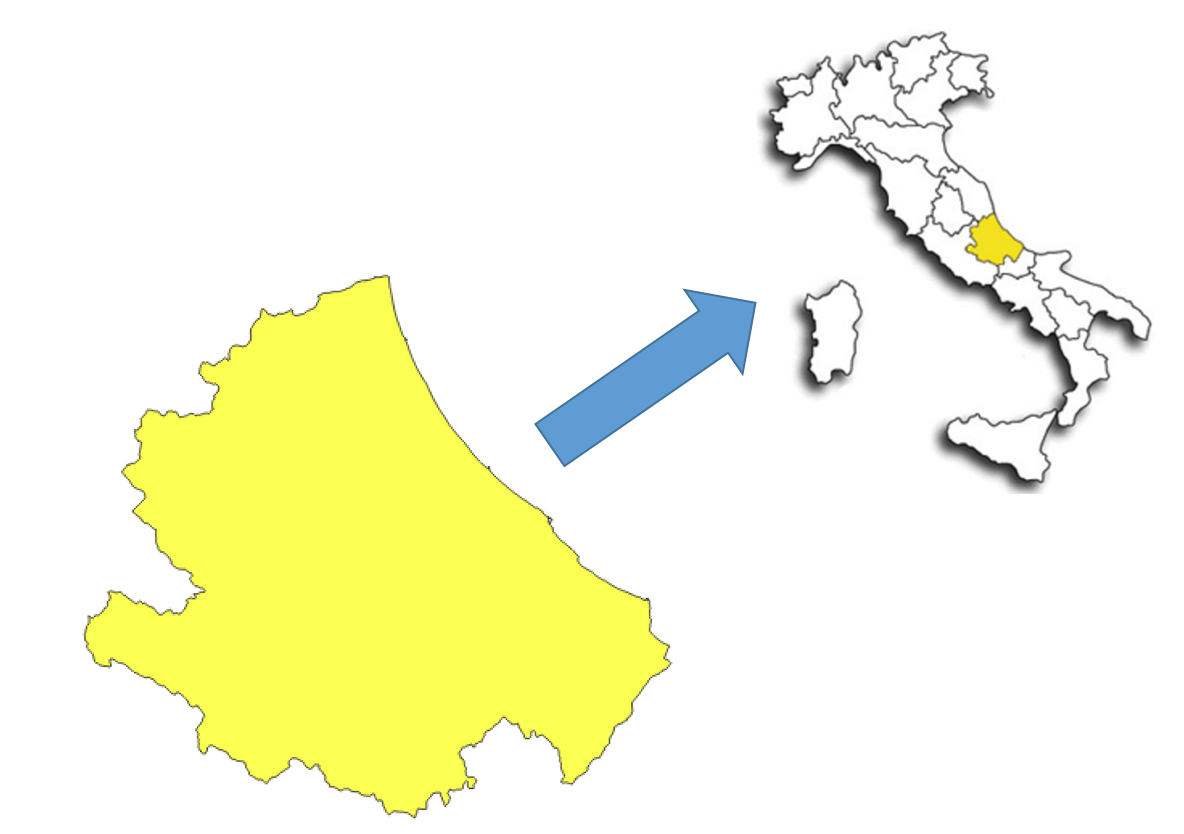
\includegraphics[width=0.5\textwidth]{img/abruzzo}
	\caption{La nostra \textit{GeoArea}: La regione Abruzzo}
    	\label{fig:abruzzo}
\end{figure}

La \textit{GeoArea} viene descritta dalla seguente tupla: <gid, geom>.
\begin{itemize}
\item \textit{gid}: Identificativo numerico univoco del territorio.
\item \textit{geom}: Rappresentazione geometrica del territorio (\textit{MultiPolygon}).
\end{itemize}
%------------------------------------------------

\item\textit{Z}=$\{${$z_k$}, k=1,2,..$\}$ dove $z_k$ denota una zona k-esima della \textit{GeoArea}, ognuna caratterizzata da un insieme di informazioni territoriali. L'insieme \textit{Z} è una partizione della \textit{GeoArea}, ovvero è una collezione di elementi $z_k$, non nulli, tali da avere intersezione vuota a due a due e tali che la loro unione coincida con l'intera \textit{GeoArea}, per maggiore chiarezza si rimanda alla fig. \ref{fig:geoarea}.  
\begin{figure}[h]
\centering
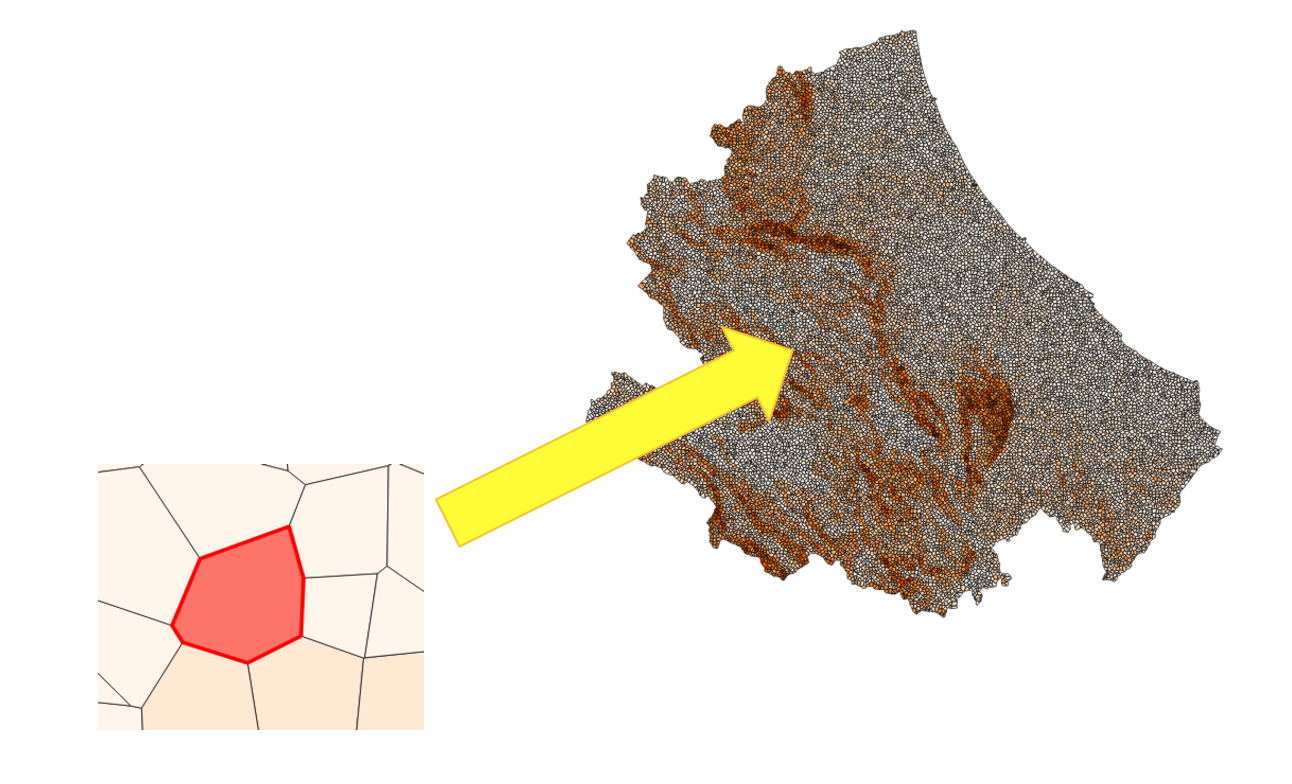
\includegraphics[width=0.5\textwidth]{img/zeta}
\caption{Generico elemento $z_k$ dell'insieme \textit{Z}}
	\label{fig:geoarea}
\end{figure}
\newpage
Il generico elemento di \textit{Z} (i.e. $z_k$) è definito mediante la tupla: <gid, $S_{zk}$, geom,\textit{avgElevation}>.
\begin{itemize}
\item \textit{gid}: Identificativo numerico univoco dell'elemento $z_k$.
\item \textit{$Sz_k$}: Valore numerico che quantifica la pericolosità di frana dell'elemento $z_k$. 
\item \textit{geom}: Rappresentazione geometrica del \textit{boundary} dell'elemento $z_k$.

\item \textit{avgElevation}: Altitudine media dell'elemento $z_k$, ottenuta mediante una media ponderata delle altitudini delle curve di livello che intersecano, almeno in parte, l'elemento $z_k$. Il modo in cui verrà calcolato questo valore verrà descritto nel dettaglio nella notazione successiva di $\Delta{h}$ poiché bisogna prima introdurre ulteriori concetti.
\end{itemize}
Si noti che $z_k$ è una notazione sovraccaricata dato che rappresenta sia il \textit{gid} della zona che la sua geometria.
%------------------------------------------------

\item\textit{B}=$\{$ $b_i$, i=1,2,... $\}$ dove $b_i$ indica l'edificio della stazione (\textit{B} sta per \textit{Station Building}) contenuta nel \textit{boundary} della \textit{GeoArea}. Di questo edificio non teniamo conto della sua conformazione architettonica, della sua altezza o del numero di piani della struttura poiché spesso sono delle informazioni che difficilmente sono reperibili ma bensì consideriamo la sua posizione geografica, espressa da una coppia di coordinate, informazione spesso nota. Un esempio di un generico elemento $b_i$ è rappresentato in fig. \ref{fig:b}.
\newpage
\begin{figure}[bht]
\centering
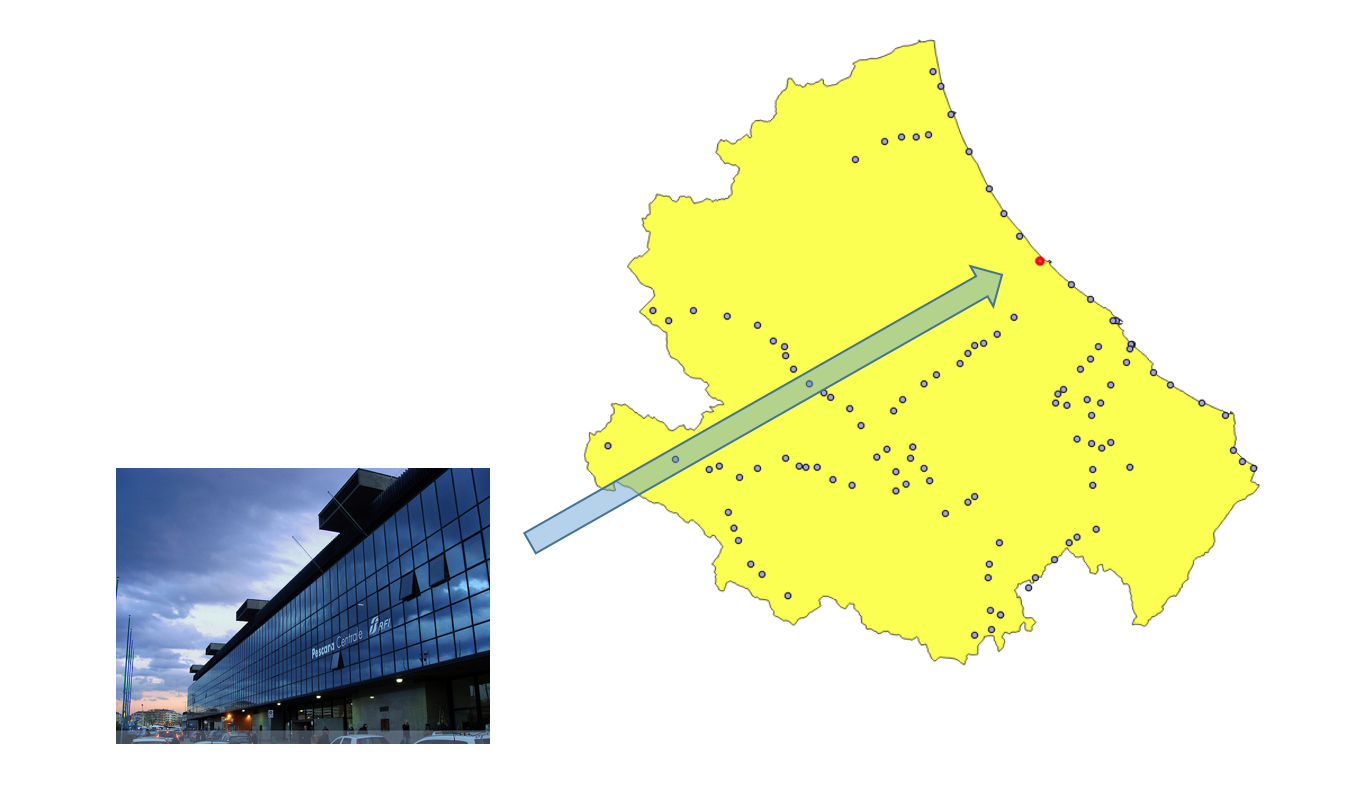
\includegraphics[width=0.5\textwidth]{img/stazionegenerica}
\caption{Generico elemento $b_i$ dell'insieme \textit{B}}
	\label{fig:b}
\end{figure}

Il generico elemento di \textit{B} (i.e. $b_i$) è definito mediante la tupla: <gid, name, geom, \textit{$Exp\_b_i$}, \textit{elevation}>.
\begin{itemize}
\item \textit{gid}: Identificativo numerico univoco dell'elemento $b_i$.
\item \textit{name}: Nome testuale dell'i-esimo elemento dell'insieme \textit{B}, espresso tramite una stringa.
\item \textit{geom}: Rappresentazione geometrica (\textit{Point}) dell'elemento $b_i$.
\item \textit{Exp$\_$$b_i$}: Grado di esposizione al pericolo di frana del generico elemento $b_i$, determinato da tutte le $z_k$ in \textit{Z}.
\item \textit{elevation}: Altitudine espressa in metri a cui si trova il generico elemento $b_i$.
\end{itemize}
Si noti che $b_i$ è una notazione sovraccaricata dato che rappresenta sia il \textit{gid} della stazione ferroviaria che la sua geometria.
%------------------------------------------------
\item\textit{E}=$\{$ $e_j$, j=1,2,... $\}$ dove $e_j$ denota una curva di livello contenuta almeno in parte nel \textit{boundary} della \textit{GeoArea}. In geografia, con particolare riguardo alla cartografia, la curva di livello è quella curva che unisce punti con uguale quota (figura 4(b)), ovvero uguale distanza verticale dal piano di riferimento al quale è stato attribuito quota zero; se sono sopra il livello del mare si chiameranno \textit{isoipse} (dal greco ísos = "uguale" e hýpsos = "altezza") mentre al contrario \textit{isobate} (dal greco ísos = "uguale" e báthos = "profondità"). Nella figura 4(a) è possibile vedere un esempio di $e_j$.

\begin{figure}[bth]
\myfloatalign
\subfloat[]
{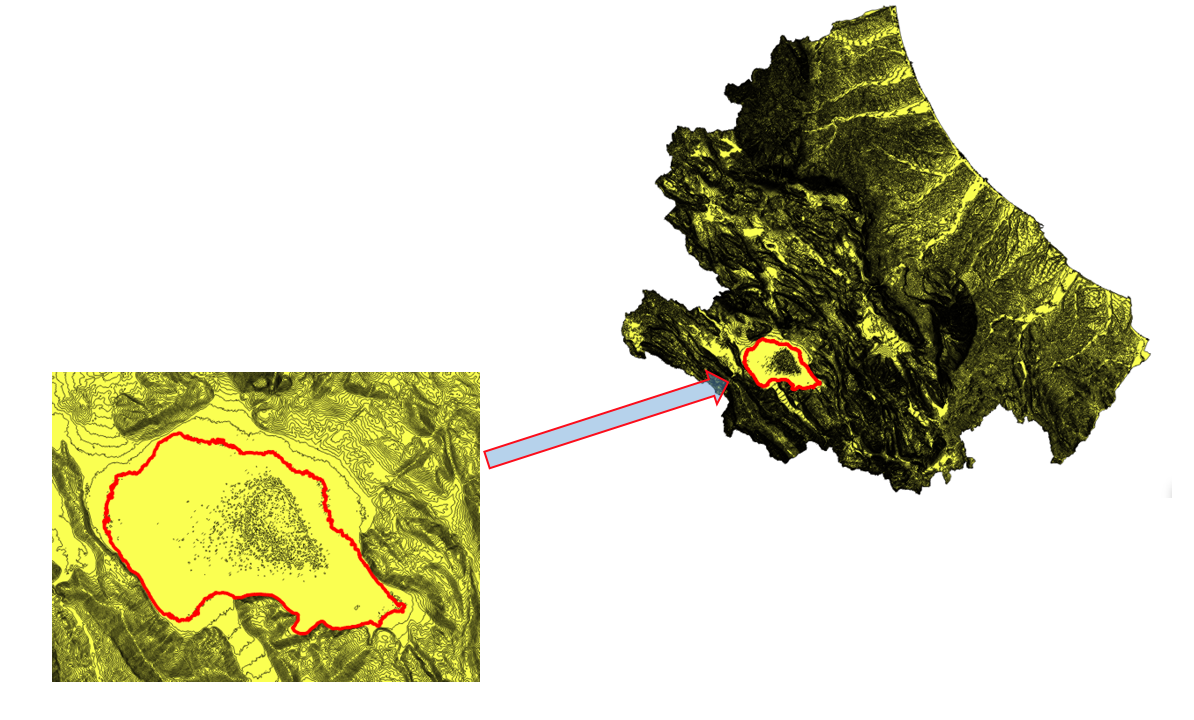
\includegraphics[width=.45\linewidth]{img/curva}} \quad
\subfloat[]
{\label{fig:example-b}
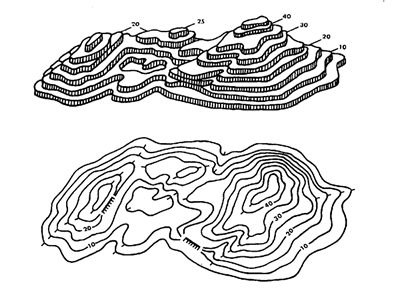
\includegraphics[width=.45\linewidth]{img/esempioLivello}} \\
\label{fig:example}
\caption{(a) Generico elemento $e_j$ dell'insieme; (b)Esempio di curve di livello per un certo territorio }
\end{figure}


Ogni elemento dell'insieme \textit{E} (i.e. $e_j$) è definito mediante la tupla: <gid, elevation, geom>.
\begin{itemize}
\item \textit{gid}: Identificativo numerico univoco dell'elemento $e_j$.
\item \textit{elevation}: Valore numerico che rappresenta la quota espressa in metri dell'elemento $e_j$.
\item \textit{geom}: Rappresentazione geometrica (\textit{MultiLineString}) dell'elemento $e_j$.
\end{itemize}
Si noti che $e_j$ è una notazione sovraccaricata dato che rappresenta sia il \textit{gid} della curva di livello che la sua geometria.
%------------

\item\textit{buffer$_i$}=buffer($b_i$,$r$) rappresenta una geometria costituita da tutti i punti la cui distanza dal punto $b_i$ risulta essere minore o uguale del raggio $r$. Nella figura \ref{fig:bufferi} è possibile vedere un esempio di $buffer_i$.
\begin{figure}[bht]
\centering
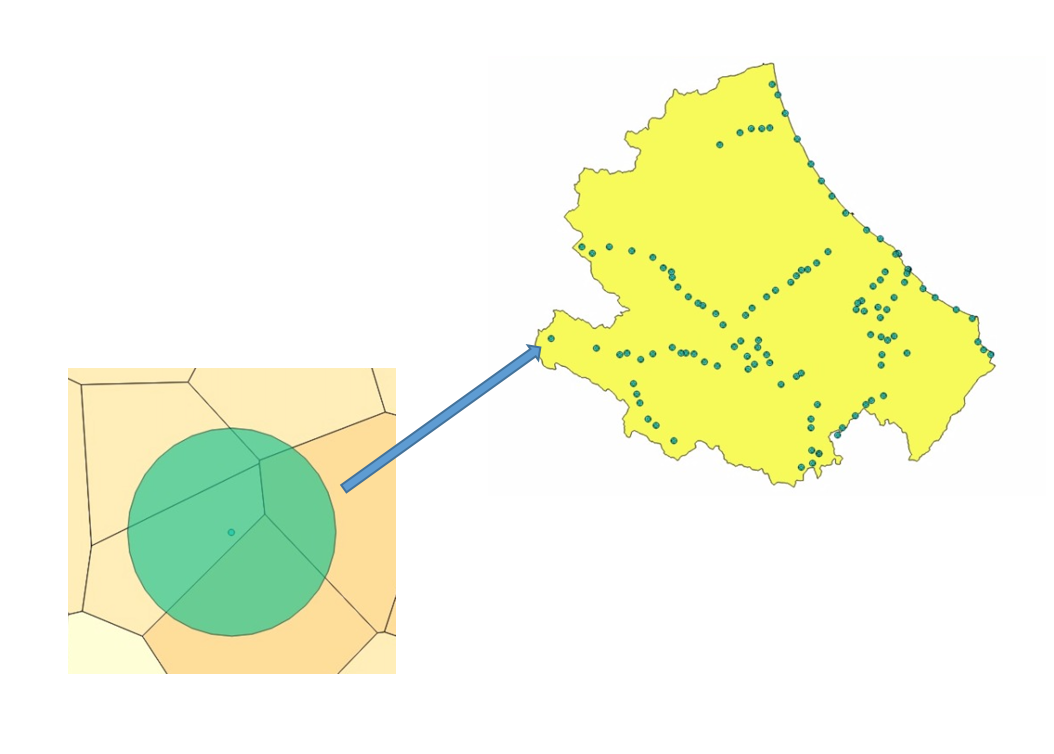
\includegraphics[width=0.5\textwidth]{img/buffer}
\caption{Esempio di $buffer_i$ costruito su una generica $b_i$}
\label{fig:bufferi}
\end{figure}
%-----------
\newpage
\item\textit{V}=$\{$$v_\gamma$ ($\gamma$=1,2,...) := $z_k$ $\in$ \textit{Z} | $buffer_i$ $\cap$ $z_k$ $\neq$ $\emptyset$ $\}$ è l'insieme di tutte le $z_k$ contenute nella \textit{GeoArea} che intersecano almeno in parte \textit{$buffer_i$}. La cardinalità di tale insieme è pari a $N$. Un esempio di insieme $V$ è osservabile nella fig. \ref{fig:v}.
\begin{figure}[bht]
\centering
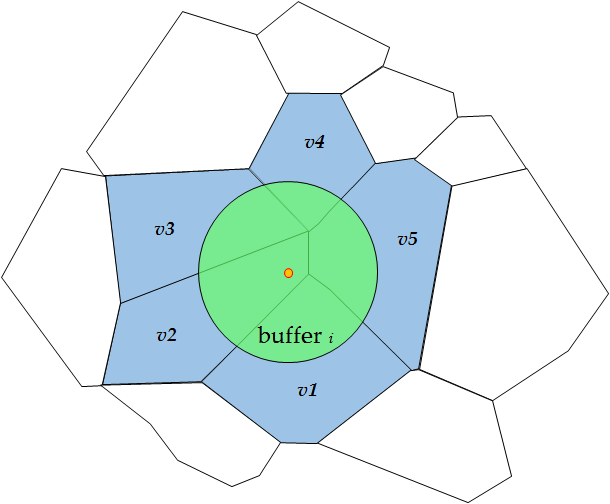
\includegraphics[width=0.5\textwidth]{img/V}
\caption{V=$\{$$v_1$, $v_2$, $v_3$, $v_4$, $v_5$ $\}$}
\label{fig:v}
\end{figure}
%-----------

\item\textit{P}=$\{$$p_m$ (m=1,2,..) := $buffer_i$ $\cap$ $e_j$ $\neq$ $\emptyset$, $\forall$ $e_j$ $\in$ \textit{E}$\}$ è l'insieme dei segmenti delle curve di livello, determinati dall'intersezione tra le curve di livello contenute nell'insieme \textit{E} e il $buffer_i$. In figura \ref{fig:p} è riportato un esempio di insieme $P$.
\begin{figure}[h]
\centering
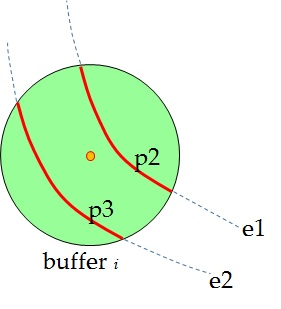
\includegraphics[width=0.4\textwidth]{img/P}
\caption{P=$\{$$p_2$, $p_3$$\}$}
\label{fig:p}
\end{figure}
%-----------
\newpage
\item\textit{T}=$\{$$t_f$ (f=1,2,...) := $v_\gamma$ $\cap$ $e_j$ $\neq$ $\emptyset$, $\forall$ $e_j$ $\in$\textit{E}, $\forall$ $v_\gamma$$\in$\textit{V}$\}$ è l'insieme dei segmenti delle curve di livello, determinati dall'intersezione tra le curve di livello contenute nell'insieme \textit{E} e le zone $v_\gamma$ contenute nell'insieme \textit{V}. In fig. \ref{fig:t} è possibile osservare un esempio di insieme T.
\begin{figure}[h]
\centering
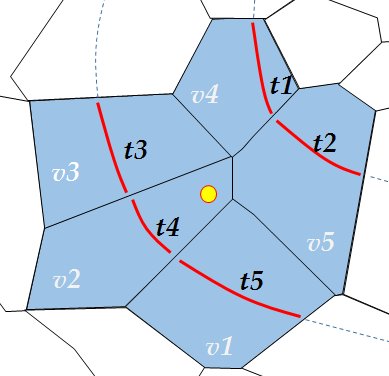
\includegraphics[width=0.4\textwidth]{img/T}
\caption{T=$\{$$t_1$, $t_2$, $t_3$, $t_4$, $t_5$ $\}$}
\label{fig:t}
\end{figure}
%-----------

\item $\Delta{h}$ è così definito:
\begin{equation}
 \Delta{h} =  | h\_stazione - h\_media\_v_\gamma |
 \end{equation}
Dove: 
\begin{itemize}
\item $ h\_stazione$ indica l'\textit{elevation} dell'edificio $b_i$
\item $ h\_media\_v_\gamma$ indica l'\textit{avgElevation} media di $v_\gamma$
\end{itemize}
Il metodo di calcolo dell'elevation per gli edifici e le zone è diverso. Infatti qui di seguito descriveremo le diverse modalità di calcolo:
\begin{enumerate}
\item h\_media\_$v_\gamma$ : l'\textit{elevation} delle v$_\gamma$ viene calcolata effettuando la media aritmetica dell'elevation delle curve di livello che intersecano $v_\gamma$.

\begin{figure}[h]
  \centering
    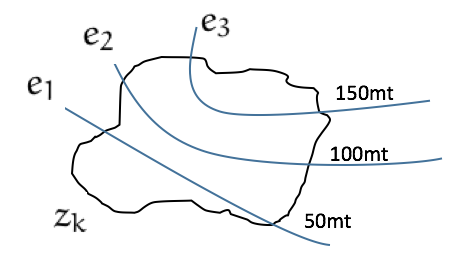
\includegraphics[width=0.5\textwidth]{img/altezzaZK}
      \caption{Esempio di una $v_\gamma$ con tre curve di livello}
      \label{fig:altezzaZK}
\end{figure}
Ad esempio, in fig.\ref{fig:altezzaZK} la quota media di $v_\gamma$ risulta essere: \newline
$\frac{50\ +\ 100\ +\ 150}{3} = 100 mt$

\item $h\_{stazione}$: il calcolo dell'\textit{elevation} per gli edifici è più sofisticato ma permette di ottenere valori molto accurati.
Le possibili situazioni che si possono presentare sono tre e verranno analizzate qui di seguito:
\begin{itemize}
\item edificio racchiuso da un'unica curva di livello (Fig.10) oppure in prossimità del confine della \textit{GeoArea} (Fig.11). Si definisce un edificio di questo tipo come edificio in posizione "atipica".

\begin{figure}[bth]
\myfloatalign
\subfloat[]
{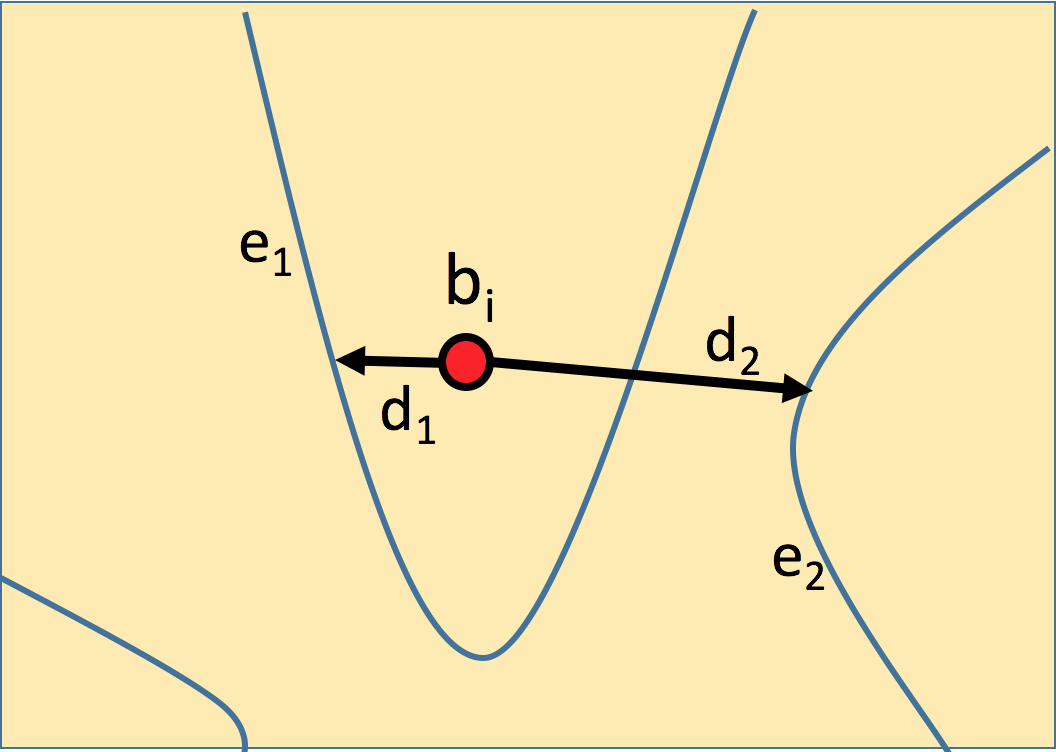
\includegraphics[width=.45\linewidth]{img/unalinea}} \quad
\subfloat[]
{\label{fig:unalinea-a}
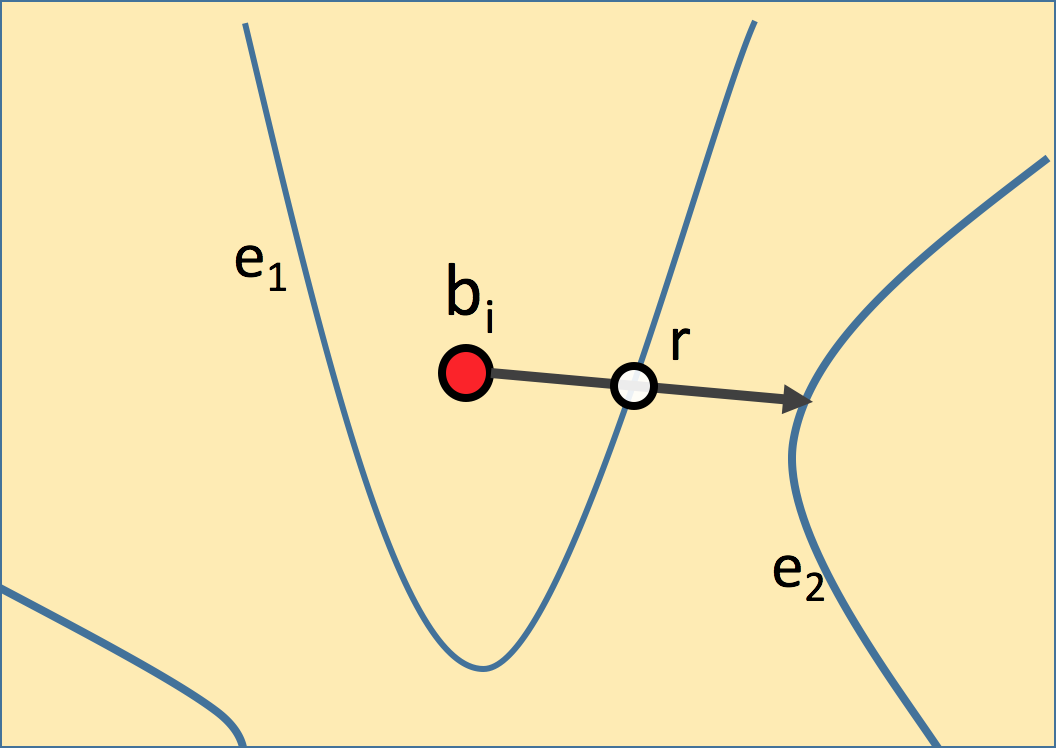
\includegraphics[width=.45\linewidth]{img/unalinea2}} 
\caption[]{Edificio racchiuso da un'unica curva di livello.}\label{fig:unalinea}
\end{figure}

\begin{figure}[bth]
\myfloatalign
\subfloat[]
{\label{fig:confine-a}
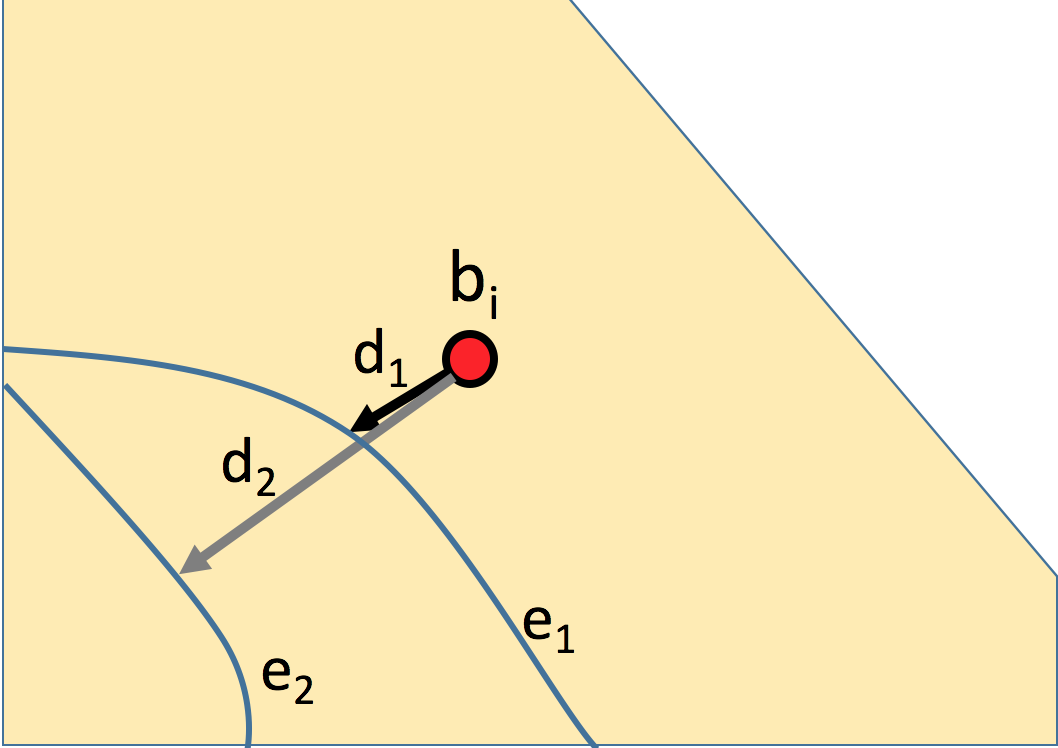
\includegraphics[width=.45\linewidth]{img/lineaconfine}} \quad
\subfloat[]
{\label{fig:confine-b}
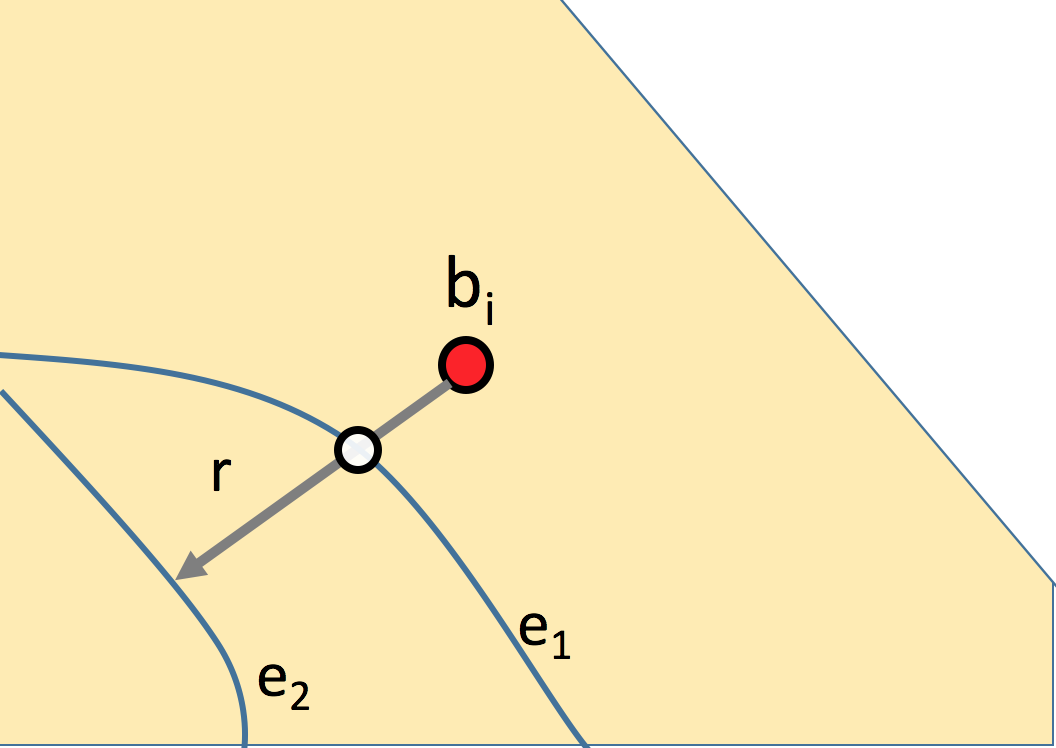
\includegraphics[width=.45\linewidth]{img/lineaconfine2}} 
\caption[]{Edificio in prossimità del confine della \textit{GeoArea}.}\label{fig:confine}
\end{figure}

Entrambi i casi vengono rilevati nel medesimo modo, ovvero tracciando la semiretta avente come origine l'edificio $b_i$ (pallino rosso) e passante per la curva $e_2$. Se la semiretta interseca anche $e_1$, allora ci troviamo in una delle situazioni esplicate in Fig.\ref{fig:unalinea} (b) e in Fig. \ref{fig:confine} (b). Quindi $h\_stazione$ equivale all'\textit{elevation} della curva di livello $e_1$, supponendo che $d_1 < d_2$.

\newpage

\item Edificio circondato da due curve di livello come in Fig.\ref{fig:circondata}. Si definisce un edificio di questo tipo come edificio in posizione "tipica".

\begin{figure}[bth]
\myfloatalign
\subfloat[]
{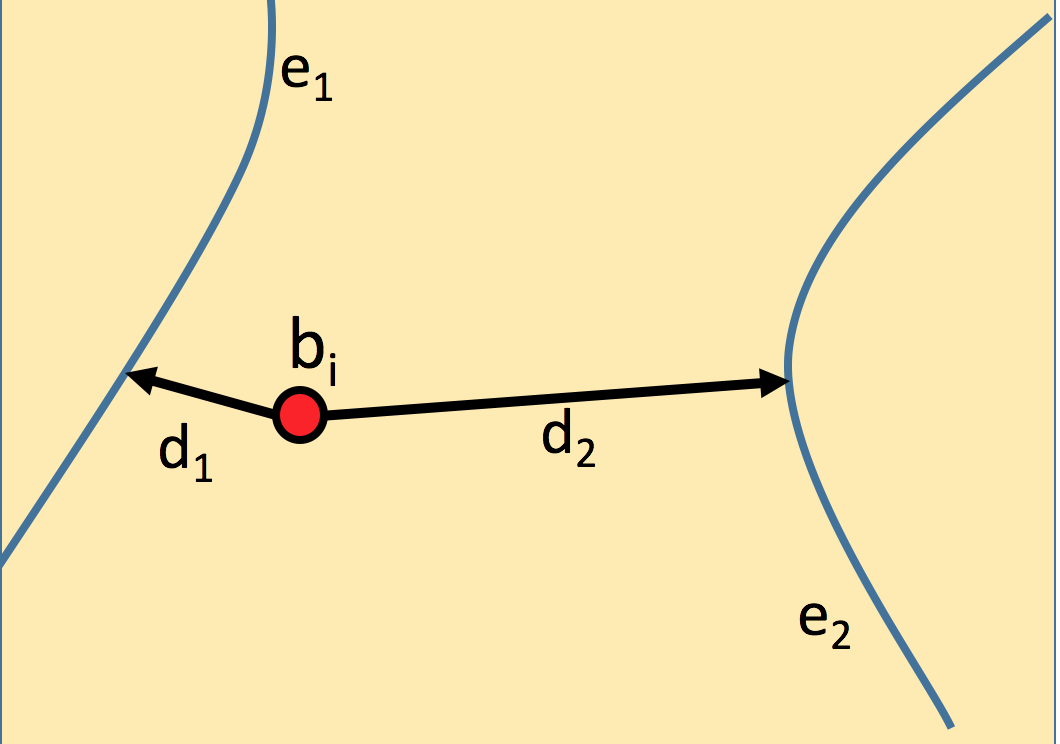
\includegraphics[width=.45\linewidth]{img/duelinee-a}} \quad
\subfloat[]
{\label{fig:circondata-b}
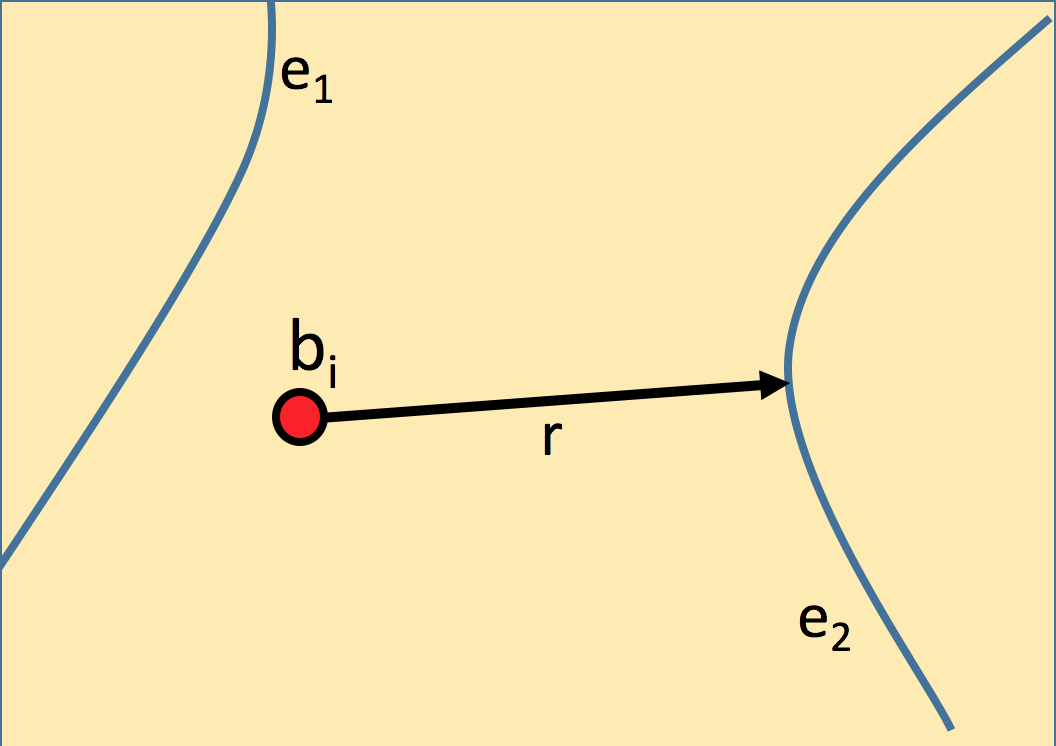
\includegraphics[width=.45\linewidth]{img/duelinee-b}} 
\caption[]{Edificio in prossimità del confine della \textit{GeoArea}.}\label{fig:circondata}
\end{figure}

Dalla Fig.\ref{fig:circondata} (b) si evince che, a differenza delle situazioni esplicate dalle Fig.\ref{fig:unalinea} (b) e Fig.\ref{fig:confine} (b), la semiretta avente origine in $b_i$ e passante per $e_2$ non interseca la curva di livello $e_1$.
Dunque $h\_stazione$ è così definito:
\begin{equation}
\label{eq:hstazione}
   h\_stazione = \frac{(h\_e_1 \times d_2) \times ( h\_e_2 \times d_1)}{d_1 +d_2}
\end{equation}
Dove:
\begin{itemize}
\item $h\_e_j$ indica l'\textit{elevation} della curva di livello $e_j$, con $j=1,2$
\item $d_j$ indica la distanza tra l'edificio $b_i$ e la curva di livello $e_j$ con $j=1,2$
\end{itemize}

L'Eq.\ref{eq:hstazione} è una media ponderata delle quote delle due curve di livello più vicine all'edificio $b_i$. Al numeratore le distanze vengono utilizzate come pesi della media, affinché la quota della curva $e_1$, più vicina all'edificio $b_i$, risulti più determinante nel calcolo della $h\_stazione$ rispetto alla quota della curva $e_2$.
\end{itemize}
\end{enumerate}

\item \textit{Azimuth}:
L'azimuth è la coordinata orizzontale angolare espressa dall'arco d'ortodromia della sfera celeste che si forma partendo convenzionalmente dal punto cardinale nord fino all'oggetto di osservazione,muovendosi in senso orario verso est, quindi a sud e a ovest, fino a tornare al punto di inizio a nord (cioè un angolo giro, 360° sessagesimali); la coordinata azimutale quindi, verrà espressa in gradi angolari sessagesimali/minuti/secondi, oppure in radianti, e avrà sempre un valore numerico positivo. Un punto nel cielo che si trovi esattamente a nord (il polo celeste dell'emisfero boreale) avrà una coordinata azimutale di 0° (o 360°), se invece si trova esattamente a est sarà di 90°, esattamente a sud di 180°, esattamente a ovest di 270°, ecc. Si propone un esempio in Fig.\ref{fig:azimuth}.

\begin{figure}[bth]
  \centering
    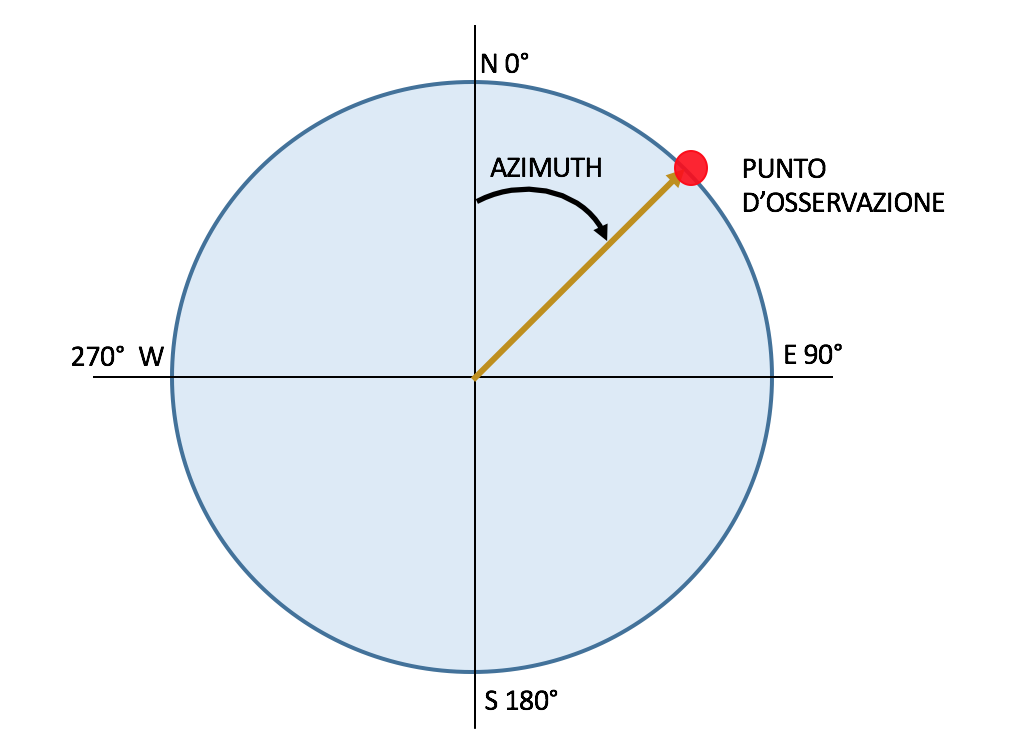
\includegraphics[width=0.6\textwidth]{img/azimuth}
      \caption{Esempio di angolo azimuth per un certo punto}
       \label{fig:azimuth}
\end{figure}



\item \textit{vettoreDirezionale}: il vettore direzionale viene così costruito:
	\begin{enumerate}
	\item trova l'\textit{Azimuth} tra $b_i$ e il punto più vicino della $p_m$ più vicina.
    \item Crea il punto $A$, le cui coordinate $(x_a,y_x)$ sono le coordinate di $b_i$ traslate di $\Delta{x}$ e $\Delta{y}$. \newline
    Dove:
    	\begin{itemize}
    		\item $\Delta{x}= cos (Azimuth) \times (r+1)$
            \item $\Delta{y}= sin (Azimuth) \times (r+1)$
    	\end{itemize}
    con $r$ pari al raggio del $buffer_i$.
    \item crea infine il \textit{vettoreDirezionale}, ovvero il vettore avente come origine $b_i$ e come punto finale il punto $A$ sopra definito.
	\end{enumerate}
    Si propone un esempio esplicativo in Fig.\ref{fig:vettore}.
  \begin{figure}[bth]
  \centering
    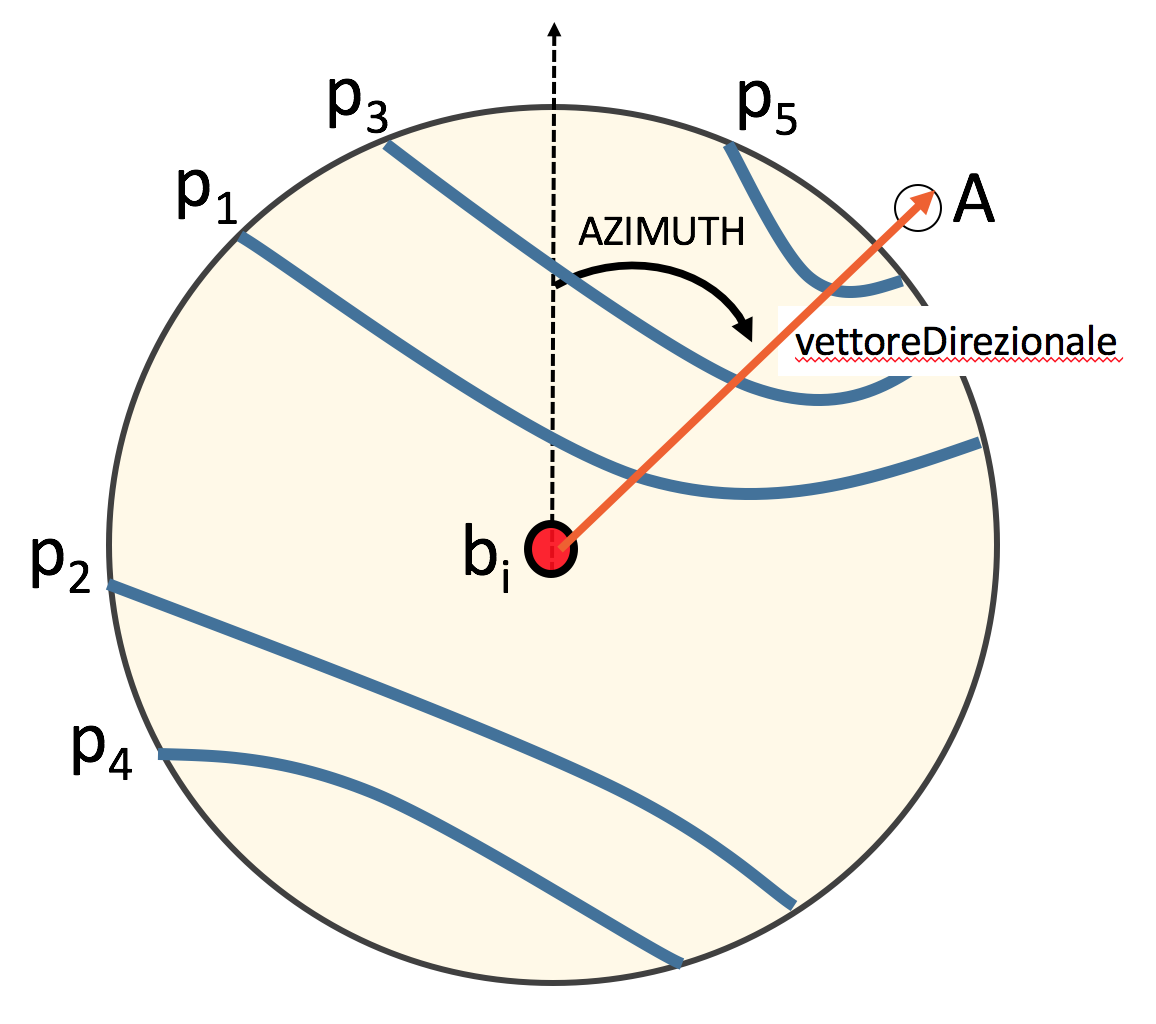
\includegraphics[width=0.5\textwidth]{img/vettore}
      \caption{Esempio di vettore direzionale per un certo edificio $b_i$}
        \label{fig:vettore}

\end{figure}
\newpage
\item \textit{Q}=$\{$ $q_w$ (w=1,2,...,$\beta$)) :=  $p_m$ $\in$ $P$ | $(p_m \cap vettoreDirezionale) \neq \emptyset$ | $d_1$<$d_2$<...<$d_\beta$ $\}$.
\newline
Dove:
\begin{itemize}
\item $d_w$ è la distanza tra $b_i$ e il punto ($p_m \cap vettoreDirezionale$) 
\end{itemize}
Per costruzione i pedici stabiliscono un ordinamento crescente degli elementi dell'insieme $Q$ rispetto la distanza appena definita.\newline
La Fig.\ref{fig:Q} propone un esempio esplicativo basato sulla Fig.\ref{fig:vettore}. Come si vede sono state escluse dall'insieme $Q$ le $p_m$ |($p_m \cap vettoreDirezionale = \emptyset$)  


\begin{figure}[bth]
  
  \centering
    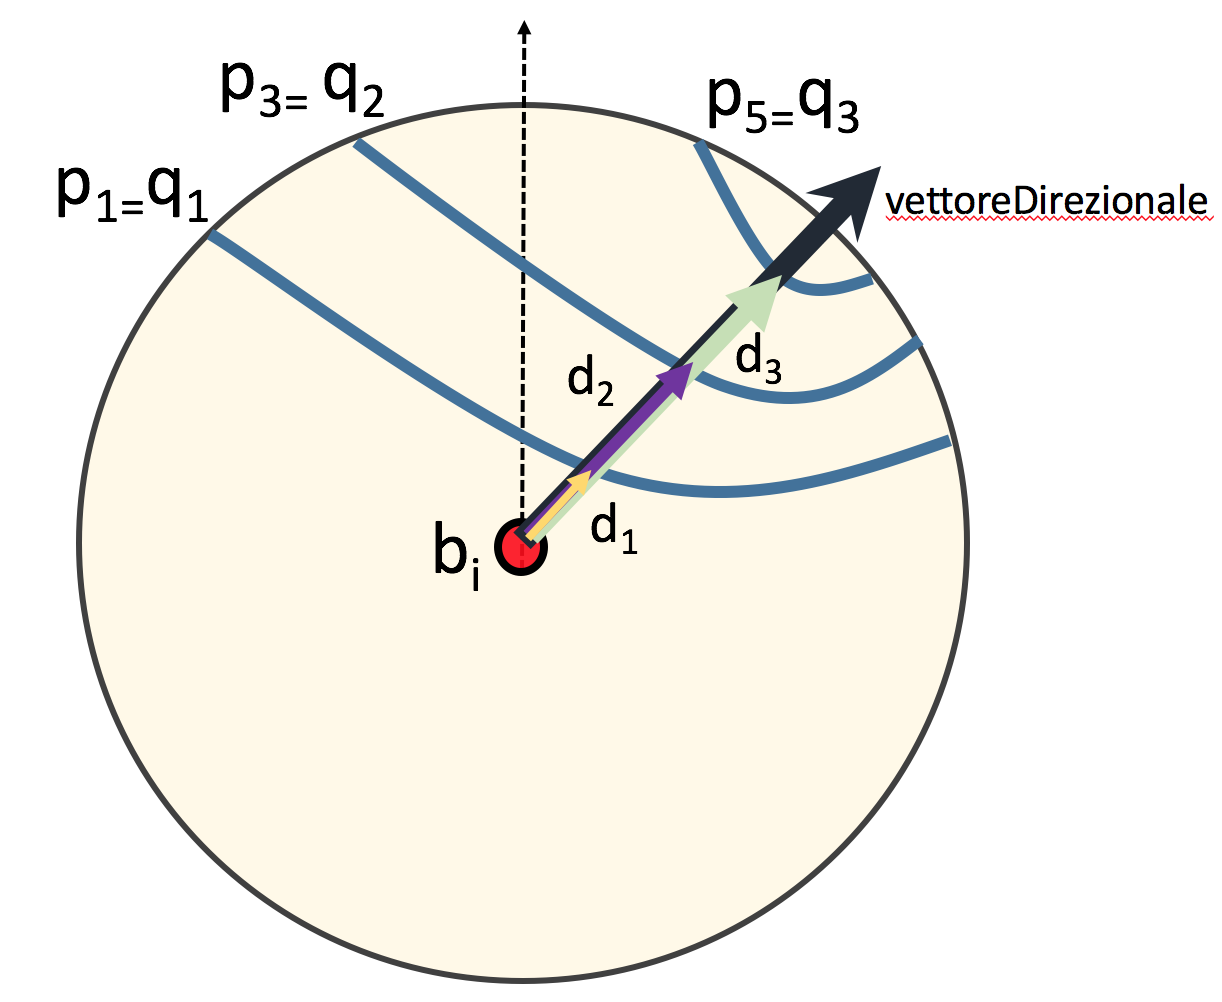
\includegraphics[width=0.5\textwidth]{img/Q}
      \caption{$Q=\{q_1,q_2,q_3\}$}
      \label{fig:Q}
\end{figure}
\newpage

\item \textit{trend}:Il trend rappresenta l'andamento del territorio nelle immediate vicinanze di $b_i$ in direzione del \textit{vettoreDirezionale}  e può assumere uno dei seguenti valori \{\textit{salita}, \textit{discesa}\}, in base alle seguenti condizioni:
\begin{itemize}
\item \textit{trend} = \textit{salita} se $elevation\_q_1 > h\_stazione$.\newline Esempio in Fig.\ref{fig:salita1}

\begin{figure}[bth]
  \centering
    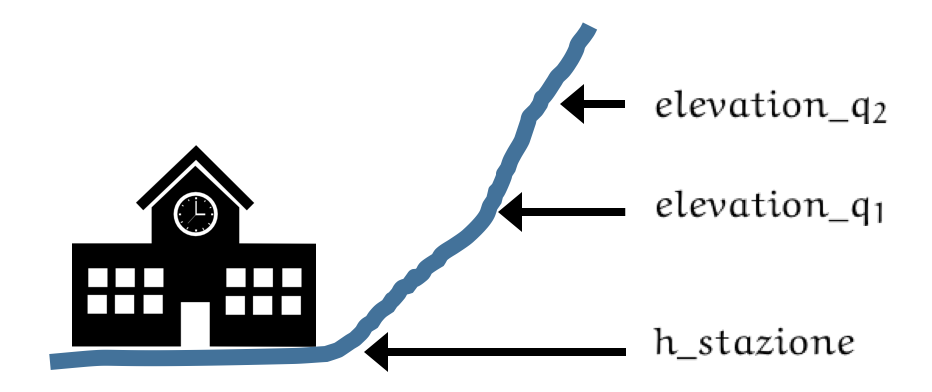
\includegraphics[width=0.8\textwidth]{img/salita1}
      \caption{Esempio di un \textit{trend}=\textit{salita} 
        \label{fig:salita1}
      nel caso in cui la stazione si trova ad una quota minore rispetto la curva di livello $q_1$}
\end{figure}

\item \textit{trend} = \textit{salita} se $elevation\_q_1 = h\_stazione$ $\wedge$ $elevation\_q_2 > elevation\_q_1$. \newline 
Esempio in Fig.\ref{fig:salita2}.
\begin{figure}[bth]
  \centering
    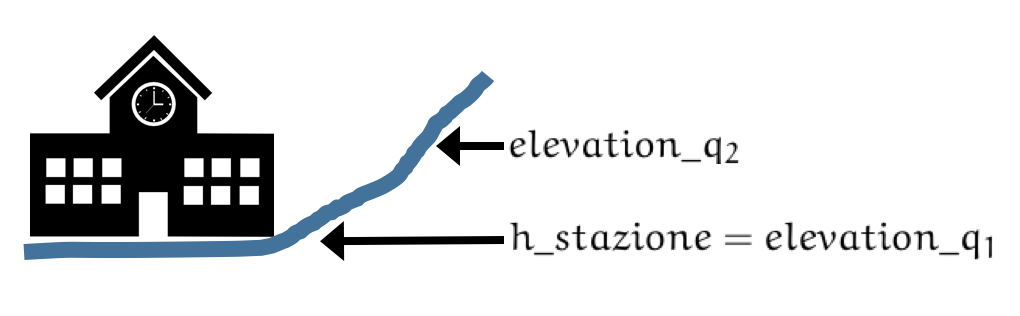
\includegraphics[width=0.8\textwidth]{img/salita2}
      \caption{Esempio di un \textit{trend} = \textit{salita}
        \label{fig:salita2}
nel caso in cui la stazione si trova alla stessa quota della curva di livello $q_1$}
\end{figure}
\newpage

\item \textit{trend} = \textit{discesa} se $elevation\_q_1 < h\_stazione$.\newline
Esempio in Fig.\ref{fig:discesa1}

\begin{figure}[bth]
  \centering
    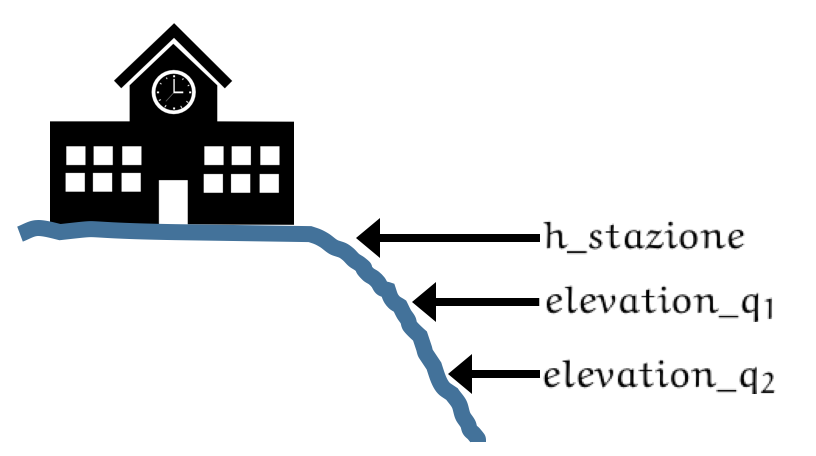
\includegraphics[width=0.8\textwidth]{img/discesa1}
      \caption{Esempio di un \textit{trend}=\textit{discesa}
      \label{fig:discesa1}
nel caso in cui la stazione si trova a quota maggiore rispetto la della curva di livello $q_1$}
\end{figure}



\item \textit{trend} = \textit{discesa} se $elevation\_q_1 = h\_stazione$ $\wedge$ $elevation\_q_2 < elevation\_q_1$.\newline
Esempio in Fig.\ref{fig:discesa2}
\begin{figure}[bth]
  \centering
    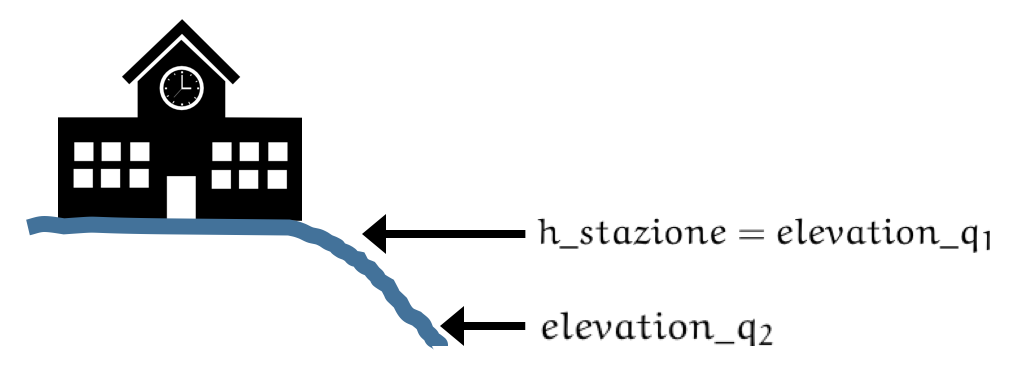
\includegraphics[width=0.8\textwidth]{img/discesa2}
      \caption{Esempio di un \textit{trend}=\textit{discesa}
        \label{fig:discesa2}
nel caso in cui la stazione si trova a quota maggiore rispetto la della curva di livello $q_1$}
\end{figure}

\end{itemize}

\item \textit{situazione Monotonica}: una situazione monotonica è garantita fino ad un certo $q_{\overline{w}}$ se:
\begin{itemize}
\item è garantita $\forall w<\overline{w}$ 
\item la differenza di $elevation$ tra $q_{\overline{w}}$ e $q_{\overline{w}-1}$ conferma l'andamento del \textit{trend}. Ovvero:
\begin{equation}
\label{monotonica}
\begin{cases}
               elevation\_q_{\overline{w}} < elevation\_q_{\overline{w}-1},  & \text{se trend = discesa}\\
               elevation\_q_{\overline{w}} > elevation\_q_{\overline{w}-1}, & \text{se trend = salita}
            \end{cases} 
\end{equation}
\end{itemize} 


\item \textit{pendenza} è una stima dell'andamento del territorio vicino l'edificio $b_i$ lungo il suo $vettoreDirezionale$ associata a q$_w$. Dal punto di vista geometrico la \textit{pendenza} rappresenta il coefficiente angolare tra due punti. In un caso tra una stazione $b_i$ e il punto ottenuto dall'intersezione tra il \textit{vettoreDirezionale} e la curva di livello $q_1$. Nell'altro caso tra i punti ottenuti dall'intersezione tra il \textit{vettoreDirezionale} e le curve $q_w$ e $q_{w+1}$. In entrambi i casi il coefficiente viene calcolato rispetto al sistema di riferimento della \textit{GeoArea}.
Come mostrato nella figura  \ref{fig:pendenza}

\begin{figure}[bth]
\myfloatalign
\subfloat[ ]
{\label{pendenza1}
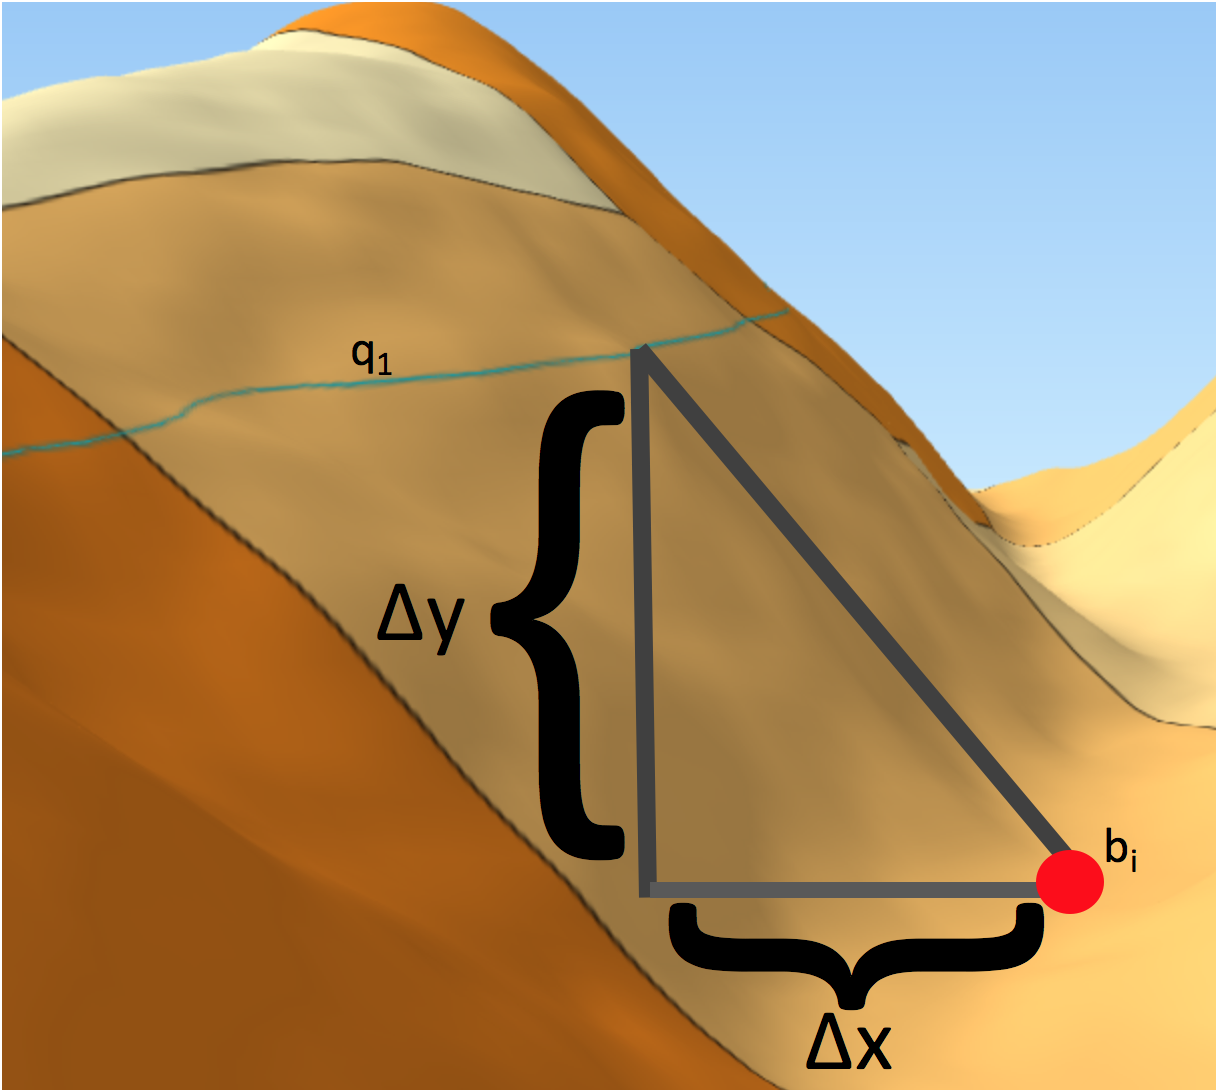
\includegraphics[width=.45\linewidth]{img/pendenza1}} \quad
\subfloat[]
{\label{pendenza2}
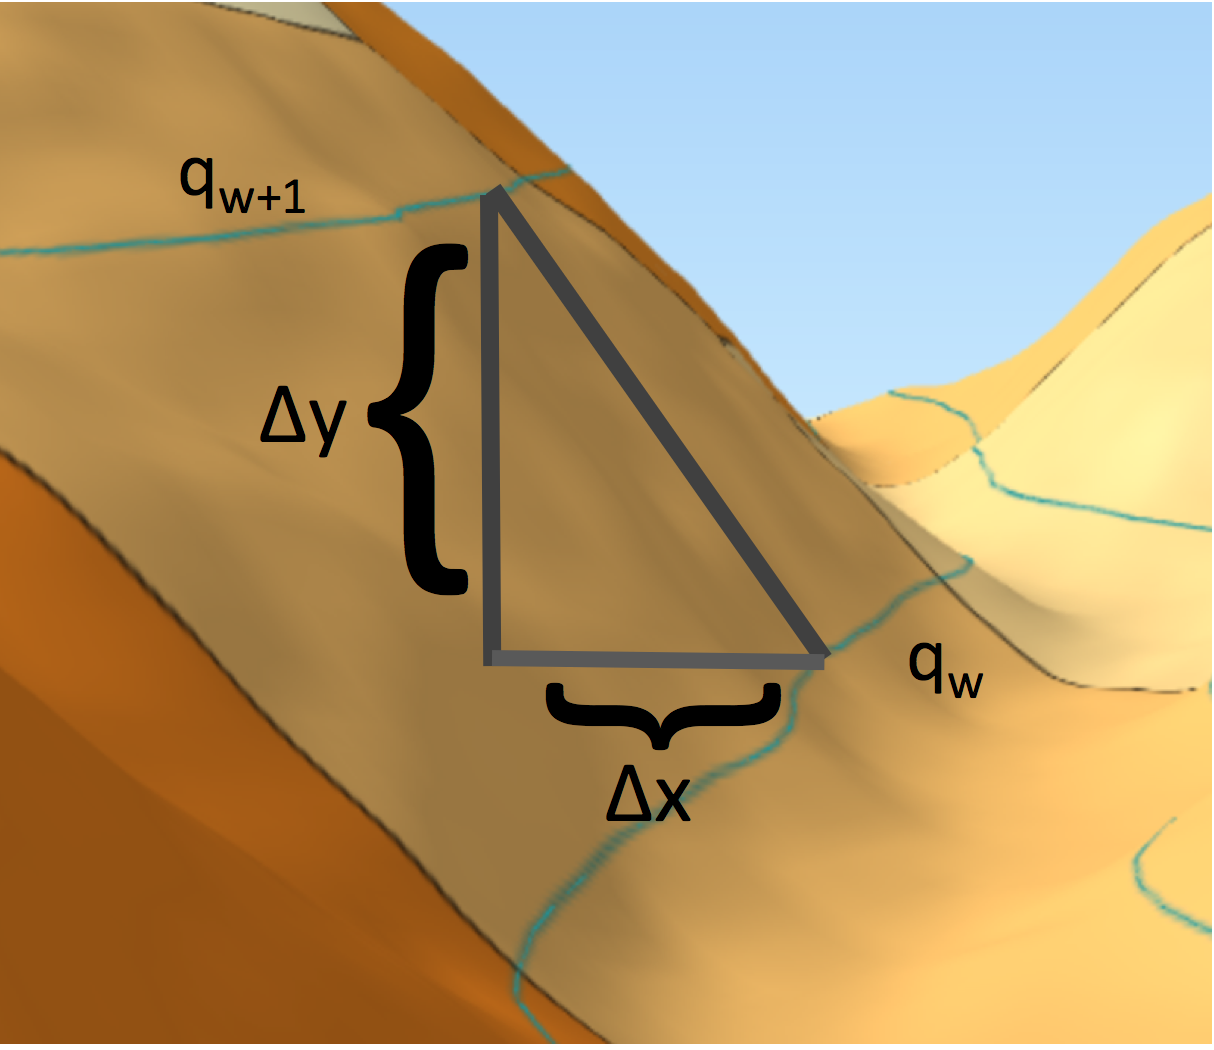
\includegraphics[width=.45\linewidth]{img/pendenza2}} 
\caption[dove]{Esempio esplicativo di \textit{pendenza}.  $\Delta$y corrisponde al numeratore  e $\Delta$x al denominatore dell'Eq.\ref{pendenza}, per $w=1$ subFig.\ref{fig:pendenza} (a) e per w$\geq$2 subFig.\ref{fig:pendenza} (b)}\label{fig:pendenza}
\end{figure}

Dal punto di vista matematico l'equazione per determinare la \textit{pendenza} è la seguente:
\begin{equation}
\label{pendenza}
\begin{cases}
     \frac{| h\_stazione - elevation\_q_w|}
     {d(b_1,(vettoreDirezionale \cap q_w))}  & \text{se w=1}\\
                \frac{| elevation\_q_w - elevation\_q_{w-1}|}
    {d((vettoreDirezionale \cap q_w),(vettoreDirezionale \cap q_{w-1}))} & \text{se w $\geq$ 2}
            \end{cases} 
\end{equation}


\item $slope_i$: E' la somma aritmetica delle \textit{pendenze} di tutti gli elementi di $Q$ che garantiscono una \textit{situazione Monotonica}.

%\item $\alpha_{slope}$: è un fattore moltiplicativo numerico intero, fissato ad un certo valore sulla base di prove sperimentali. Ha lo scopo di eliminare alcuni falsi positivi/negativi.



\end{enumerate}
 

%----------------------------------------------------------------------------------------

\section{Un metodo per classificare le stazioni ferroviarie}


\subsection{Metodo di calcolo originario}
\label{metodoVecchio}
Prima di procedere con l'ideazione di un metodo di calcolo, si è pensato di effettuare un'analisi critica e dettagliata del metodo originario, frutto del lavoro di altri studenti negli anni passati.
Supponiamo di avere quindi una \textit{GeoArea} partizionata in zone diverse e indicate con $z_k$, ognuna delle quali ha associato un valore $s_{zk}$ rappresentante il pericolo di frana. Si ricorda che tali notazioni sono già state introdotte in \ref{notazioni}.
Tale metodo assegna un valore di \textit{exposure} ($Exp_{bi}$) ad un generico edificio ($b_i$) all'interno della \textit{GeoArea} nel seguente modo:
\begin{enumerate}

\item L'\textit{Explosure} per l'edificio $b_i$ è ottenuto come somma dei contributi di tutte le zone nella \textit{Geoarea} per tale edificio.
\begin{equation}
\label{sum_exp_old}
 Exp$\_$b_i = \sum\limits_{k=1}^{\overline{N}}  Exp$\_$b_{i,k}
\end{equation}

\item Il contributo della generica zona $z_k$ all'\textit{exposure} dell'edificio $b_i$ viene calcolato utilizzando la seguente equazione:\newline
\begin{equation}
\label{equazioneVecchia}
Exp$\_$b_i,k = \overline{Size} \times S_{z_k} \times  \begin{cases}
               1,  & \text{se $b_i$ è contenuta in $z_k$}\\
               \frac{1}{d^3}, & \text{altrimenti}
            \end{cases} 
\end{equation}

Dove:
\begin{itemize}
\item \textit{$\overline{Size}$} è il rapporto tra l'area di $z_k$ e l'area media di tutte le zone che costituiscono $Z$
\item \textit{d} denota la distanza minima tra $b_i$ e il \textit{boundary} della zona $z_k$
\end{itemize}
Al prodotto di questi due parametri viene poi moltiplicato un certo valore in base alla posizione relativa tra la zona $z_k$ e l'edificio $b_i$. Tale valore corrisponderà ad 1 se vi è una situazione analoga alla figura seguente:

\begin{figure}[bth]
  \label{fig:stazDentro}
  \centering
    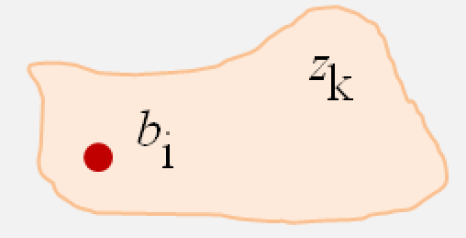
\includegraphics[width=0.5\textwidth]{img/stazDentro}
      \caption{Esempio di un edificio $b_i$ all'interno di una zona                    $z_k$}
\end{figure}

Se invece l'edificio $b_i$ si trova esternamente rispetto alla zona $z_k$, il valore sarà $\frac{1}{d^3}$.

\begin{figure}[bth]
  \label{fig:stazDentro}
  \centering
    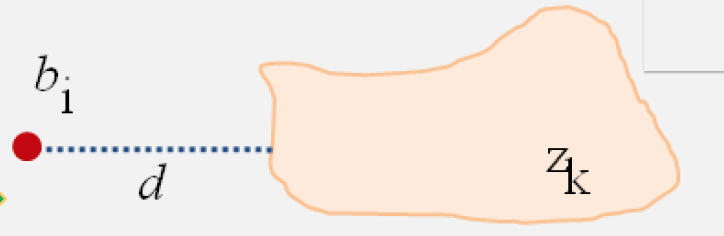
\includegraphics[width=0.5\textwidth]{img/stazFuori}
      \caption{Esempio di un edificio $b_i$ esterno alla zona                    $z_k$}
\end{figure}
\end{enumerate}

Detto ciò possiamo concludere questa breve panoramica sul metodo di calcolo originario con alcune critiche e considerazioni, che hanno rappresentato la base per la realizzazione di un nuovo metodo:
\begin{itemize}
\label{controMetodoVecchio}
\item Il metodo non tiene conto delle curve di livello che cadono nella \textit{GeoArea};
\item Il valore del parametro \textit{Size} è vicino allo zero per zone molto piccole, mentre è maggiore di 1 per tutte le zone che hanno area superiore al valore dell’area media delle zone della \textit{GeoArea}. Inoltre \textit{Size} assume valori molto alti per zone con area molto estesa.
\end{itemize}


\subsection{Metodo di calcolo ex novo}
\label{metodoNuovo}
Il metodo proposto vuole sostituirsi a quello precedente, vedi \ref{metodoVecchio}, con lo scopo di migliorare il calcolo dell'\textit{exposure}. Ovvero si vogliono assegnare valori che rappresentino con maggiore fedeltà il pericolo reale di frana per gli edifici. 
Il punto di forza del nuovo metodo, d'ora in avanti indicato con \textit{NMC}, consiste nello sfruttare il "potenziale informativo" aggiuntivo fornito con l'introduzione delle \textbf{curve di livello}. \newline




Viene da sé che un uso "intelligente" di queste curve, permette di ricavare importanti informazioni ai fini del nostro obiettivo, tra le quali:
\begin{itemize}
\item La quota dell'edificio
\item La morfologia del territorio
\end{itemize}
Supponiamo per un attimo di essere riusciti a ricavare queste informazioni e di averle utilizzate in modo corretto, il \textit{NMC} avrebbe così superato la prima debolezza del metodo originario, vedi \ref{controMetodoVecchio}.
Tuttavia rimarrebbero due questioni in sospeso, ovvero:
\begin{enumerate}
\label{domande}
\item Quali zone $z_k$ della \textit{GeoArea} influiscono realmente sul calcolo dell'\textit{exposure} del generico edificio $b_i$?
\item Supposto di aver trovato risposta al punto precedente, in che proporzione tali zone influiscono? tutte allo stesso modo?
\end{enumerate}
Il metodo originario, rispondeva in parte a queste domande ( vedi equazione \ref{equazioneVecchia}). \newline 
Utilizzando il parametro  $( \frac{1}{d^3} )$  si riusciva a rendere nullo il contributo di zone $z_k$ abbastanza lontane, in quanto la funzione al cubo inversa smorza rapidamente, rispondendo così alla prima domanda.\newline 
Per quanto riguarda il secondo punto, si utilizzava il parametro \textit{Size}, questo però porta alla generazione di falsi positivi/negativi nel calcolo dell'\textit{exposure} dell'edificio, come già sottolineato nel paragrafo precedente.\newline
Dunque vediamo come il \textit{NMC} ricava le informazioni dalle curve di livello e come le utilizza nel calcolo delle \textit{exposure} degli edifici $b_i$. 
\newline
L'equazione del \textit{NMC} che determina il valore finale di \textit{exposure} per la generica $b_i$ è la seguente:
\begin{equation}
\label{sum_exp_nuova}
 Exp\_b_i = (\sum\limits_{\gamma=1}^N  Exp_{bi,\gamma}) + (slope_i \times \alpha_{slope})
\end{equation}
Tale valore dipende dalla somma di due addendi. \newline
Il primo addendo rappresenta la sommatoria dei contributi delle zone $v_\gamma$ $\in$ $V$, ovvero la sommatoria degli \textit{Exp$\_$b$_{i,\gamma}$}. Si ricorda che il limite superiore $N$ della sommatoria nell'Eq.\ref{sum_exp_nuova} si riferisce al numero di zone $v_\gamma$ $\in$ $V$, ovvero alla cardinalità dell'insieme \textit{$V$}. \newline \newline
La formula per calcolare il contributo della zona $v_\gamma$ alla determinazione del pericolo di frana dell'edificio $b_i$ è la seguente:
\begin{equation}
\label{equazioneNuova}
Exp$\_$b_{i,\gamma} = Size \times S_{v_\gamma} \times \Delta{h} \times \begin{cases}
               1,  & \text{se $b_i$ è contenuta in $v_\gamma$ }\\
               \frac{1}{d}, & \text{altrimenti}
            \end{cases} 
\end{equation}
Si notino le differenze rispetto l'equazione del metodo originario ( vedi Eq.\ref{sum_exp_old}). \newline
Nella versione proposta dal \textit{NMC} il parametro ($\frac{1}{d}$) non è elevato al cubo. Questo per evitare di smorzare troppo il contributo delle $v_\gamma$ vicine. Il parametro $Size$ è così definito:
\begin{equation}
\label{size}
 Size= \frac{area (buffer_i \cap v_\gamma)}{area(v_\gamma)} 
\end{equation}

Ovvero l’area della geometria restituita dall’intersezione tra il poligono ($v_\gamma$) e il $buffer_i$ che come abbiamo definito nelle notazioni ha raggio $r$ ed è costruito attorno all'edificio $b_i$. Per un dato valore del raggio $r$, il valore del numeratore dell’Eq. \ref{equazioneNuova} cresce se la posizione di $b_i$ si avvicina al centroide della zona che lo contiene (ovvero $v_\gamma$), di conseguenza, in base all’Eq.\ref{sum_exp_nuova}, anche il corrispondente valore
dell’exposure sarà più alto.

\begin{figure}[bth]
  \label{fig:exBuffer}
   \centering
    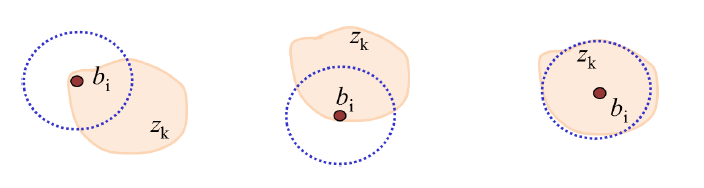
\includegraphics[width=0.8\textwidth]{img/exBuffer}
     \caption{Esempio di un edificio all'interno di una zona $v_\gamma$}
      
\end{figure}
Il parametro \textit{Size} risponde alle domande che ci siamo posti precedentemente (vedi \ref{domande}), ovvero:
\begin{itemize}
\item Quali zone $z_k$ della \textit{GeoArea} influiscono realmente sul calcolo dell'\textit{exposure} di $b_i$? E' facile ora rispondere a questa domanda, tutte e sole le zone $v_\gamma$, ovvero come abbiamo già detto le zone $z_k$ per le quali vale:
\begin{equation}
\label{sizeNotZero}
   area (buffer (b_i,r) \cap z_k) \neq \emptyset
\end{equation}
Bisogna stabilire quanto deve essere il valore del raggio, infatti se tale valore è sufficientemente grande da garantire che eventi franosi a distanza maggiore da $b_i$ non interessino quest'ultimo, allora le zone $z_k$ che non intersecano il $Buffer$ non devono contribuire al calcolo dell'\textit{exposure}. \newline


\item In che proporzione tali zone $v_\gamma$ influiscono? Tutte allo stesso modo? Ovviamente no. Grazie all'espressione \ref{size}, il parametro $Size$ tiene conto anche dell'area effettivamente occupata da $v_\gamma$ all'interno del buffer. In questo modo si riduce notevolmente la probabilità che il \textit{NMC} generi falsi positivi/negativi. \newline 



\end{itemize}


Tale parametro rappresenta, in modo quantitativo, un ulteriore legame tra l'Eq.\ref{equazioneNuova} e la morfologia del territorio. Vediamo un esempio concreto della sua utilità. \newline
La figura \ref{fig:exHmediaAlta} è stata estrapolata mediante il software di visualizzazione di dati territoriali QGIS e mostra una particolare situazione.\newline
La sfera rossa rappresenta un edificio mentre la circonferenza in blu il $buffer$, di cui abbiamo ampiamente parlato, di raggio $r$ pari a $500mt$.

\begin{figure}[bth]
  \centering
  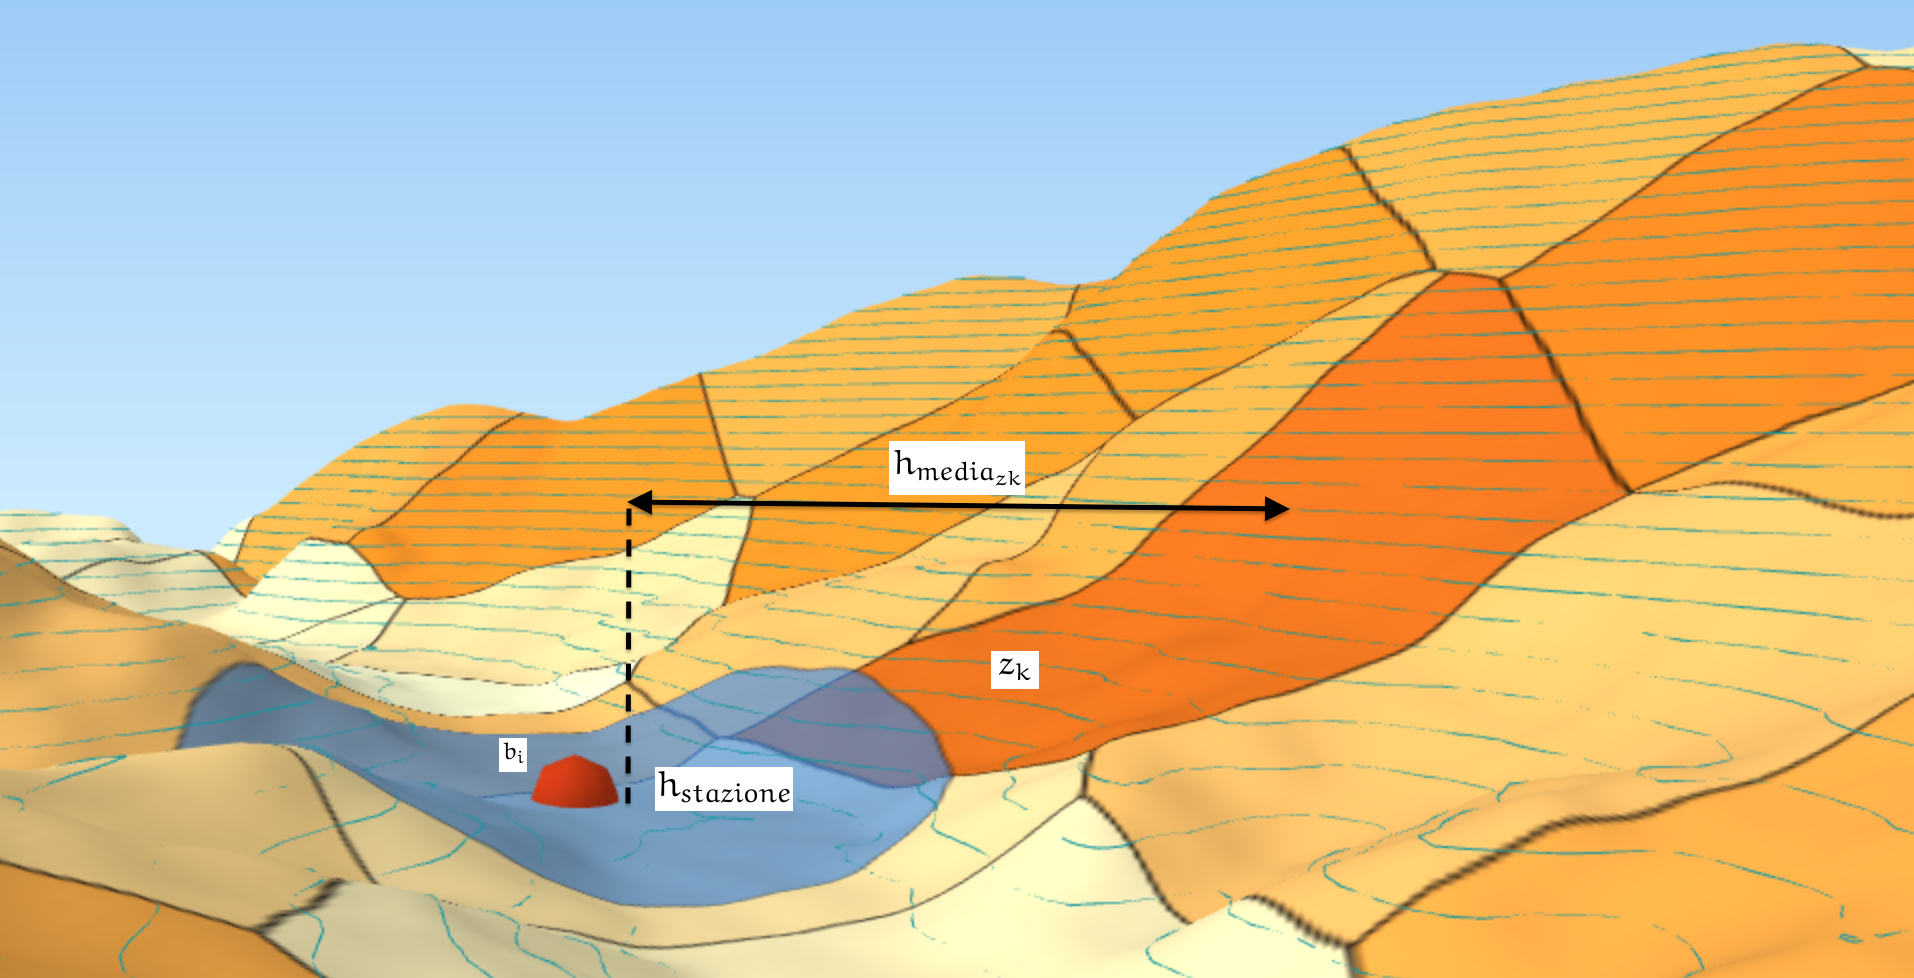
\includegraphics[width=0.8\textwidth]{img/exDeltaH}
  \caption{Esempio di una $v_\gamma$ con $h\_media\_v_{\gamma}$ elevata la cui intersezione con il $buffer_i$ risulta essere un'area piccola } 
  \label{fig:exHmediaAlta}
\end{figure}

Notiamo come la $v_\gamma$ in questione occupi una parte molto piccola del $buffer_i$. Questo sicuramente porterà ad avere un valore di $Size$ molto basso e di conseguenza anche il contributo di $v_\gamma$ all'\textit{exposure}, generando un falso negativo. Il fattore $\Delta{h}$ interviene in soccorso di $Size$, permettendo all' $Exp_{bi,\gamma}$ di assumere in valore non eccessivamente basso, tenendo conto dell'elevata differenza tra l'altezza della stazione $b_i$ e l'altezza media di $v_\gamma$.

Il secondo addendo dell'Eq.\ref{sum_exp_nuova} va a rappresentare un fattore di rischio dovuto al dislivello che si trova più vicino a b$_i$ e che quindi va considerato con maggior peso.\\ 
$\alpha_{slope}$ è un fattore moltiplicativo intero utilizzato per incrementare o diminuire il peso  di $slope_i$ nel calcolo di $Exp\_b_i$ rispetto al primo addendo.\\ 
%Sperimentalmente si osserva che ponendo $\alpha_{slope}$ pari ad 1 il contributo di $slope_i$ viene quasi trascurato mentre ponendolo pari a 10 questo va a sovrastare il contributo del primo addendo. Un valore che rappresenta un buon compromesso tra le precedenti situazioni è $\alpha_{slope}$ = 5.  

 

%----------------------------------------------------------------------------------------

\subsection{L'algoritmo}

Lo scopo di questo paragrafo è formalizzare gli algoritmi che implementa \textit{NMC}, descritto nella sezione 2.2.2 .\\ 
\newline
\newline
\textbf{Algoritmo 1}\\
\newline
Il primo algoritmo denominato $averageElevationNearZones$ ha come obiettivo quello di calcolare il valore di $avgElevation$ associato ai v$_\gamma$ in \textit{V}. Prende come parametri di input gli insiemi \textit{Z}, \textit{E} e l'elemento buffer$_i$ mentre restituisce come output l'insieme \textit{V}.\\

\begin{algorithm}[H]
	
	\SetKwData{Left}{left}\SetKwData{This}{this}\SetKwData{Up}{up}
	\SetKwFunction{Union}{Union}\SetKwFunction{FindCompre
ss}{FindCompress}
	\SetKwInOut{Input}{Input}\SetKwInOut{Output}{Output}

	\IncMargin{1em}
	\Input{\textit{Z}, \textit{E}, buffer$_i$}
	\Output{\textit{V}}
	\KwResult{Calcola la quota media delle zone che intersecano il buffer}
	\caption{averageElevationNearZones}
	\label{alg:one}
	\BlankLine
	
	\SetAlgoNoLine
	\textit{V}=$\emptyset$; \\
    avgElevation = $0$; \\
    contatore = $0$; \\
    
	\For{each z$_k$ $\in$ \textit{Z}}{
    	\If{z$_k$ $\cap$ \textit{buffer$_i$}}{
        	\For{each e$_j$ $\in$ \textit{E}}{
            	\If{z$_k$ $\cap$ e$_j$}{
                $avgElevation$ = $avgElevation$ + ( $elevation$ di e$_j$ ); \\
                $contatore$ = $contatore$ + 1; \\
                }
            }
            \If{contatore > $0$}{
    			$avgElevation$ = $avgElevation$/$contatore$;
    		}
			aggiorna il valore $avgElevation$ di z$_k$;\\
            v$_\gamma$ = z$_k$;\\
    		\textit{V} = \textit{V} $\cup$  v$_\gamma$;\\ 
            avgElevation = $0$; \\
    		contatore = $0$; \\
        }  
    }
	return \textit{V}; 
	

\end{algorithm}

\mbox{}\\
Commenti:\\
Dalla riga 1 alla 3 sono presenti alcune inizializzazioni: l'insieme \textit{V} inizialmente è vuoto, mentre sono fissati a $0$ i valori di $avgElevation$ e $contatore$. Dalla riga 4 alle 21 è presente un ciclo che scandisce gli elementi z$_k$ di \textit{Z}. Immediatamente all'interno del ciclo (righe 5-20) viene effettuato un controllo che verifica se la zona in esame ha un'intersezione con il buffer.\\ 
In caso di esito negativo si passa subito al successivo elemento di \textit{Z}. In caso di esito positivo, per ogni elemento e$_j$ in E, si verifica se interseca con la zona z$_k$ in esame. Se anche questo controllo viene superato si incrementa il valore di $avgElevation$ con l'$elevation$ di e$_j$ e il valore di $contatore$ di 1.\\
Una volta completato il ciclo sugli elementi in \textit{E}, si controlla (riga 12) se $contatore$ ha un valore maggiore di zero, quindi se almeno per una linea e$_j$ è verificata l'intersezione con la z$_k$ esaminata. In questo caso il valore di $avgElevation$ viene sovrascritto a $avgElevation/contatore$.\\
Si passa quindi (riga 15) ad aggiornare il valore $avgElevation$ nella tupla z$_k$ con il valore appena calcolato.\\
Alla riga 16 la tupla z$_k$ viene copiata nella tupla v$_\gamma$ che viene inserita nell'insieme \textit{V}. Questa operazioni viene eseguita per mantenere nell'insieme \textit{V} solo gli elementi z$_k$ di interesse, ossia quelli per cui è verificata l'intersezione con $buffer_i$.\\  
Alle righe 18 e 19 le variabili $avgElevation$ e $contatore$ sono resettate a $0$, per poter essere appropriatamente riutilizzate nella successiva iterazione del ciclo.\\
L'algoritmo infine (riga 22) restituisce l'insieme \textit{V}.\\
\mbox{}\\
Riassumendo l'algoritmo prende tutte e sole le z$_k$ che intersecano il buffer e per ognuna calcola la quota media. Inserisce infine queste zone nell'insieme \textit{V} che restituisce come risultato.\\
La complessità computazionale dell'algoritmo è data dal ciclo in riga 4 e da quello in riga 6. È quindi pari a $\mathcal{O}(card(\textit{Z}) \times card(\textit{E}))$ anche se mediamente è molto inferiore in quanto è molto improbabile che ogni elemento in \textit{Z} intersechi con buffer$_i$ e con tutte le linee in \textit{E}. 
\mbox{}\\
\newline
\newline
\textbf{Algoritmo 2}\\
\newline
L'algoritmo denominato $elevationBuild$ ha come obiettivo quello di stimare l'$elevation$ di b$_i$. Prende come parametri di input gli insiemi \textit{V} (l'insieme delle zone che intersecano buffer$_i$), \textit{E} (l'insieme delle curve di livello) e l'elemento b$_i$. In output restituisce lo stesso elemento b$_i$ di input il cui campo $elevation$ è stato aggiornato con la stima calcolata.\\ 

\begin{algorithm}[H]
	
	\SetKwData{Left}{left}\SetKwData{This}{this}\SetKwData{Up}{up}
	\SetKwFunction{Union}{Union}\SetKwFunction{FindCompre
ss}{FindCompress}
	\SetKwInOut{Input}{Input}\SetKwInOut{Output}{Output}

	\IncMargin{1em}
	\Input{\textit{V}, \textit{E}, b$_i$}
	\Output{\textit{b$_{i}$}}
	\KwResult{Calcola una stima dell'elevation di b$_i$}
	\caption{elevationBuild}
	\label{alg:one}
	\BlankLine
	
	\SetAlgoNoLine
	
    \textit{T}=$\emptyset$; \\
	\For{each v$_{\gamma}$ $\in$ \textit{V}}{
    	\For{each e$_j$ $\in$ \textit{E}}{
        	\If{v$_{\gamma}$ $\cap$ e$_j$}{
            	$geom$ di t$_f$ = st\_intersection ( v$_{\gamma}$, e$_j$ );\\
                $elevation$ di t$_f$ = $elevation$ di e$_j$; \\
            	\textit{T}=\textit{T} $\cup$ t$_f$;
            }
    	}
    }
    \For{each t$_f$ $\in$ \textit{T}}{
    	$dist$ = st\_distance ( b$_i$, t$_f$ );\\
        Trova t$_{fmin}$  t.c. $dist$ è minima;\\
        Trova t$_{fmin2}$   t.c. $dist$ è la successiva al minimo; \\
    }
    \If{b$_i$ in posizione atipica}{
		t$_{fmin2}$ = t$_{fmin}$;\\
    }
    Calcola $h\_stazione$ \\
    Aggiorna $elevation$ di b$_i$ con $h\_stazione$;\\
	return b$_{i}$; \\
	

\end{algorithm}

\mbox{}\\
Commenti:\\
Nella prima riga dell'algoritmo l'insieme \textit{T} è inizializzato come insieme vuoto.\\ 
Nelle righe 2-10 è presente un ciclo annidato. Il ciclo più esterno itera sugli elementi v$_\gamma$ in \textit{V} (l'insieme delle zone che intersecano il buffer), mentre quello più interno sugli elementi e$_j$ in \textit{E} (l'insieme delle linee di livello). Se l'intersezione tra gli elementi v$_\gamma$ e e$_j$ esiste, allora questa intersezione viene assegnata come geometria di t$_f$ mentre come sua $elevation$ viene assegnata l'elevation di e$_j$. L'ennupla t$_f$ così definita è inserita nell'insieme \textit{T} (riga 7). \\
All'interno del ciclo in riga 11 si vanno a scandire i t$_f$ in \textit{T}. All'interno del ciclo si va a calcolare la distanza $dist$ tra l'elemento t$_f$ e b$_i$. Si vanno quindi a individuare (nelle righe 13-14) t$_{fmin}$ e t$_{fmin2}$.\\
t$_{fmin}$ è la t$_f$ $\in$ \textit{T} tale che la distanza $dist$ tra  t$_f$ e b$_i$ è la distanza minima tra tutte le distanze calcolate tra ogni altra t$_f$ $\in$ \textit{T} e b$_i$.\\
In modo analogo t$_{fmin2}$ è la t$_f$ $\in$ \textit{T} la cui distanza $dist$ tra  t$_f$ e b$_i$ ha un valore immediatamente successivo alla distanza minima.\\
Alla riga 16 si effettua un controllo per verificare se b$_i$ si trova in una posizione "atipica" come definito nella sezione 2.1. Nel caso di esito positivo si copia l'ennupla t$_{fmin}$ in t$_{fmin2}$.\\
Si calcola quindi alla riga 19 il valore di $h\_stazione$ come descritto precedentemente (in sezione 2.1), dove t$_fmin$ rappresenta da e$_1$, mentre t$_{fmin2}$ rappresenta e$_2$.\\
Nella riga 20 si aggiorna l'$elevation$ di b$_i$ con il valore appena calcolato $h\_stazione$. Viene infine restituiti b$_i$.\\
\mbox{}\\
Riassumendo l'algoritmo individua i segmenti di linea frutto dall'intersezione tra tutte le linee in \textit{E} e le zone in \textit{V} e li inserisce nell'insieme \textit{T}. Individua poi i 2 elementi in \textit{T} che sono più vicini a b$_i$. Sfruttando questi 2 elementi calcola $h\_stazione$ cioè una stima dell'elevation di b$_i$.\\
La complessità computazionale è data dal ciclo annidato in riga 2 ed è pari a $\mathcal{O}(card(\textit{V}) \times card(\textit{E}))$ anche se mediamente è molto inferiore in quanto è molto improbabile che ogni elemento in \textit{V} intersechi tutte le linee in \textit{E}.\\ 
\mbox{}\\
\newpage
\textbf{Algoritmo 3}\\
\newline
L'algoritmo denominato $slopeFactor$ ha come obiettivo quello di calcolare lo $slope$ associato a b$_i$. Prende come parametri di input l'insieme \textit{E} delle curve livello e l'elemento buffer$_i$, mentre restituisce $slope_i$ ossia lo slope associato a b$_i$.\\ 

\begin{algorithm}[H]
	
	\SetKwData{Left}{left}\SetKwData{This}{this}\SetKwData{Up}{up}
	\SetKwFunction{Union}{Union}\SetKwFunction{FindCompre
ss}{FindCompress}
	\SetKwInOut{Input}{Input}\SetKwInOut{Output}{Output}

	\IncMargin{1em}
	\Input{\textit{E}, buffer$_i$}
	\Output{\textit{slope$_{i}$}}
	\KwResult{Calcola lo $slope$ associato a b$_i$}
	\caption{slopeFactor}
	\label{alg:one}
	\BlankLine
	
	\SetAlgoNoLine
	
    \textit{P}=$\emptyset$; \\
    \textit{Q}=$\emptyset$; \\
    slope$_i$ = $0$;\\
    \For{each e$_j$ $\in$ \textit{E}}{
    	\If{buffer$_i$ $\cap$ e$_j$}{
        	$geom$ di p$_m$ = st\_intersection ( buffer$_i$, e$_j$ );\\
            $elevation$ di p$_m$ = elevation di e$_j$;\\
            \textit{P} = \textit{P} $\cup$ p$_m$;\\
        }
    }
    Calcola il $vettoreDirezionale$;\\
    \For{each p$_m$ $\in$ \textit{P}}{
    	\If{p$_m$ $\cap$ $vettoreDirezionale$}{
        	Calcola la distanza tra b$_i$  e (p$_m$ $\cap$ $vettoreDirezionale$);\\
        	Aggiorna $distance$ di p$_m$ con la distanza calcolata;\\
            q$_w$ = p$_m$;\\
            Q = Q $\cup$ q$_w$ ;\\
        }
    }
    \For{each q$_w$ $\in$ \textit{Q} ordinato rispetto a $distance$}{
		slope$_i$ = slope$_i$ + (pendenza associata a q$_w$);
    }

	return slope$_{i}$; \\
	

\end{algorithm}
\mbox{}\\
Commenti:\\
Nelle prime righe (1-3) vengono inizializzati gli insiemi \textit{P}, \textit{Q} come insiemi vuoti e la variabile $slope_i$ a zero.\\
Dalla riga 4 inizia un ciclo che scandisce gli elementi e$_j$ in \textit{E} e per ognuno controlla se interseca con buffer$_i$. Se questa intersezione esiste, questa viene assegnata come geometria di p$_m$ mentre come sua $elevation$ viene assegnata l'$elevation$ di e$_j$. La tupla p$_m$ così definita, viene inserita nell'insieme \textit{P}. Queste operazioni permettono di lavorare su un insieme che è molto più piccolo di \textit{E} e che contiene solo le porzioni di linee di interesse.\\
Alla riga 11 viene calcolato il $vettoreDirezionale$ come definito nella sezione 2.1.\\
Nella righe 12-19 è presente un ciclo che scandisce gli elementi p$_m$ in \textit{P} e per ognuno verifica se interseca con il $vettoreDirezionale$. Se questa intersezione esiste viene calcolata la distanza tra b$_i$ e l'intersezione. Il valore di distanza calcolato va ad aggiornare il valore $distance$ in p$_m$. La tupla p$_m$  così costruita viene quindi copiata in q$_w$. Alla riga 17, q$_w$ viene inserito nell'insieme  \textit{Q}. In questo modo in \textit{Q} si vanno a inserire tutti e soli gli elementi p$_m$ che intersecano il $vettoreDirezionale$. \\
Nella riga 20 inizia un ciclo che scandisce gli elementi q$_w$ in \textit{Q} ordinati rispetto al campo $distance$. All'interno del ciclo viene calcolata la pendenza associata a q$_w$ come definita nelle sezione 2.1. Questo valore va a incrementare slope$_i$.\\ 
Viene infine restituito slope$_i$.\\
\mbox{}\\
Riassumendo l'algoritmo individua le porzioni di linee di livello che si trovano tutte in una stessa direzione rispetto a b$_i$ e per ognuna di esse calcola la pendenza, ossia la ripidità tra la linea e la linea precedente, dove la linea precedente è più vicina a b$_i$. slope$_i$ è la somma di queste pendenze.\\
La complessità computazionale è data dal ciclo in riga 4 ed è quindi pari a $\mathcal{O}(card(\textit{E}))$.\\
\mbox{}\\
\newpage
\textbf{Algoritmo 4}\\
\newline
L'algoritmo denominato $computeExplosure$ è l'algoritmo che effettivamente calcola l'$explosure$ associato a b$_i$. All'interno dell'algoritmo vengono richiamati tutti e tre gli algoritmi precedentemente definiti.\\

\begin{algorithm}[H]
	
	\SetKwData{Left}{left}\SetKwData{This}{this}\SetKwData{Up}{up}
	\SetKwFunction{Union}{Union}\SetKwFunction{FindCompre
ss}{FindCompress}
	\SetKwInOut{Input}{Input}\SetKwInOut{Output}{Output}

	\IncMargin{1em}
	\Input{\textit{B}, $r$, $\alpha_{slope}$, \textit{E}, \textit{Z}}
	\Output{\textit{B}}
	\KwResult{Calcola l'$explosure$ di tutte le  b$_i$}
	\caption{computeExplosure}
	\label{alg:one}
	\BlankLine
	
	\SetAlgoNoLine
	
    \For{each b$_i$ $\in$ \textit{B}}{
    	buffer$_i$ = st\_buffer( b$_i$, $r$ );\\
        \textit{V} = averageElevationNearZones ( \textit{Z}, \textit{E}, buffer$_i$ );\\
        b$_i$ =  elevationBuild ( \textit{V}, \textit{E}, b$_i$ );\\
        slope$_i$ = slopeFactor ( \textit{E}, b$_i$, buffer$_i$);\\
        \For{each v$_\gamma$ $\in$ \textit{V}}{
        	Calcola $Size$;\\
            Calcola $Exp\_b_{i,\gamma}$;\\
        }
        Calcola $Exp\_b_i$;\\
        Aggiorna il valore di $Exp\_b_i$ in b$_i$;\\
    }


	return \textit{B}; \\
	

\end{algorithm}
\mbox{}\\
Commenti:\\
Nelle righe 1-11 è presente un ciclo che scandisce tutte le b$_i$ in B.
Per ogni b$_i$ viene calcolato un buffer circolare di raggio $r$.  Viene successivamente costruito un insieme \textit{V}  che contiene tutte le zone che intersecano il buffer, dove a ogni zona viene associata una quota media (richiamando l'algoritmo 1).\\ 
Nella riga 4 la tupla b$_i$ viene aggiornata inserendo un valore che rappresenta una stima della sua quota (richiamando l'algoritmo 2).\\
Nella riga 5 viene quindi calcolato slope$_i$ (richiamando l'algoritmo 3).\\
Dalla riga 6 inizia un ciclo che scandisce gli elementi in \textit{V} e per ognuno calcola $Size$ e Exp\_b$_{i,\gamma}$.\\
In riga 10 si calcola $Exp\_b_i$ (tenendo conto anche del fattore $\alpha_{slope}$ come mostrato nell'Eq.\ref{sum_exp_nuova}) che va ad aggiornare il valore nella tupla b$_i$.\\
L'algoritmo ritorna come risultato l'insieme \textit{B} dove ogni tupla b$_i$ viene arricchita con un stima della quota e un valore di $Explosure$. 
\mbox{}\\
La complessità computazionale è data dai due cicli presenti alle righe 1 e 10 ed è quindi pari a $\mathcal{O}(card(\textit{V}) \times card(\textit{B}))$. \\
\mbox{}\\





\section{Un metodo per classificare le linee ferroviarie}
Il metodo proposto per classificare le stazioni (vedi Sez.\ref{metodoNuovo}) può essere utilizzato anche per classificare le linee ferroviarie. Occorre tuttavia estendere il NMC a causa della diversa rappresentazione geometrica dei due elementi.


\subsection{Metodo di calcolo}
\label{metodoLinee}
Poiché il NMC è stato progettato per classificare stazioni,  rappresentate attraverso dei punti geometrici, non può essere utilizzato così com'è per classificare le linee ferroviarie rappresentate invece attraverso linee geometriche. Di seguito in Fig.\ref{lineeFerroviarie} un esempio di tratta ferroviaria.

\begin{figure}[bth]
  \centering
  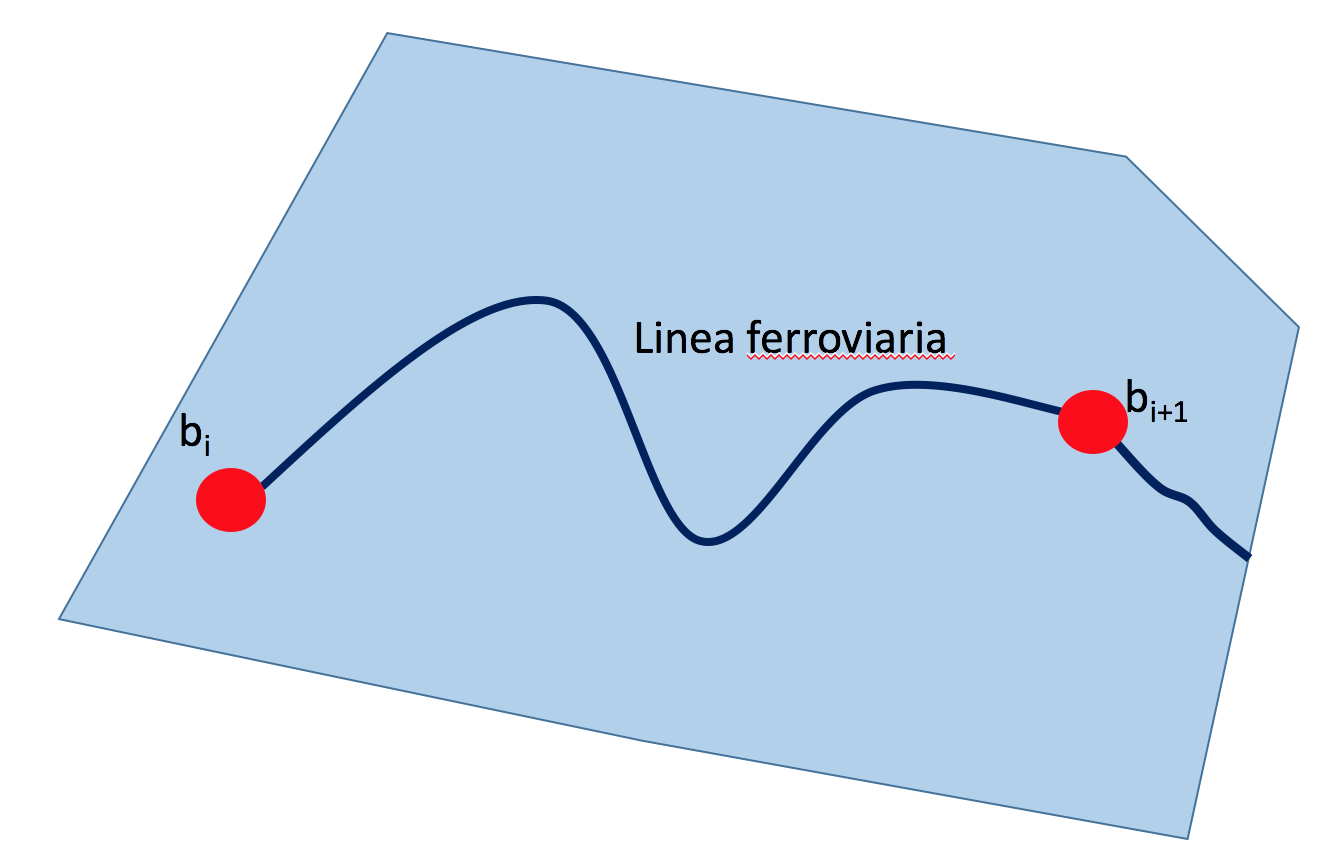
\includegraphics[width=0.7\textwidth]{img/lineaFerroviaria}
  \caption{Esempio di rappresentazione geometrica di una linea ferroviaria } 
  \label{lineeFerroviarie}
\end{figure}
L'idea di fondo è campionare con un certo passo, le linee ferroviarie. Fatto ciò si avrà una sequenza di punti sui quali poter applicare il NMC. \newline
Nonostante l'idea sembri essere molto semplice, ci sono tre questioni sulle quali bisogna fare delle riflessioni e proporre delle soluzioni:
\begin{enumerate}
\item che passo di campionamento? la scelta di un passo piccolo giova alla correttezza del calcolo finale di \textit{exposure} della tratta ma aumenta significativamente i tempi di esecuzione del calcolo stesso.
\item le linee sono semplici? le linee ferroviarie potrebbero avere delle traiettorie complesse, il metodo deve essere in grado di gestirle.
\item come aggregare i punti campionati? dopo aver campionato una certa tratta e aver determinato i valori di \textit{exposure} di ogni punto della sequenza che la compongono, bisognerà aggregare in qualche modo tali risultati per poter aver un risultato utile e consultabile.  
Il campionamento potrebbe generare un numero considerevole di punti che presi singolarmente non forniscono un contributo significato al problema in questione ( vedi \ref{ch:introduzione})
\end{enumerate}
L'estensione del NMC (d'ora in avanti indicato con NMCE) per le linee ferroviarie propone una soluzione per ognuna di queste problematiche. Nell'ordine in cui sono state precendetemente presentate: 
\begin{enumerate}
\item Il passo di campionamento scelto è di 300 mt, ma può essere facilmente modificato essendo un parametro del metodo. Di seguito in Fig.\ref{puntiLinea} un esempio di campionamento.
\begin{figure}[bth]
	\centering
	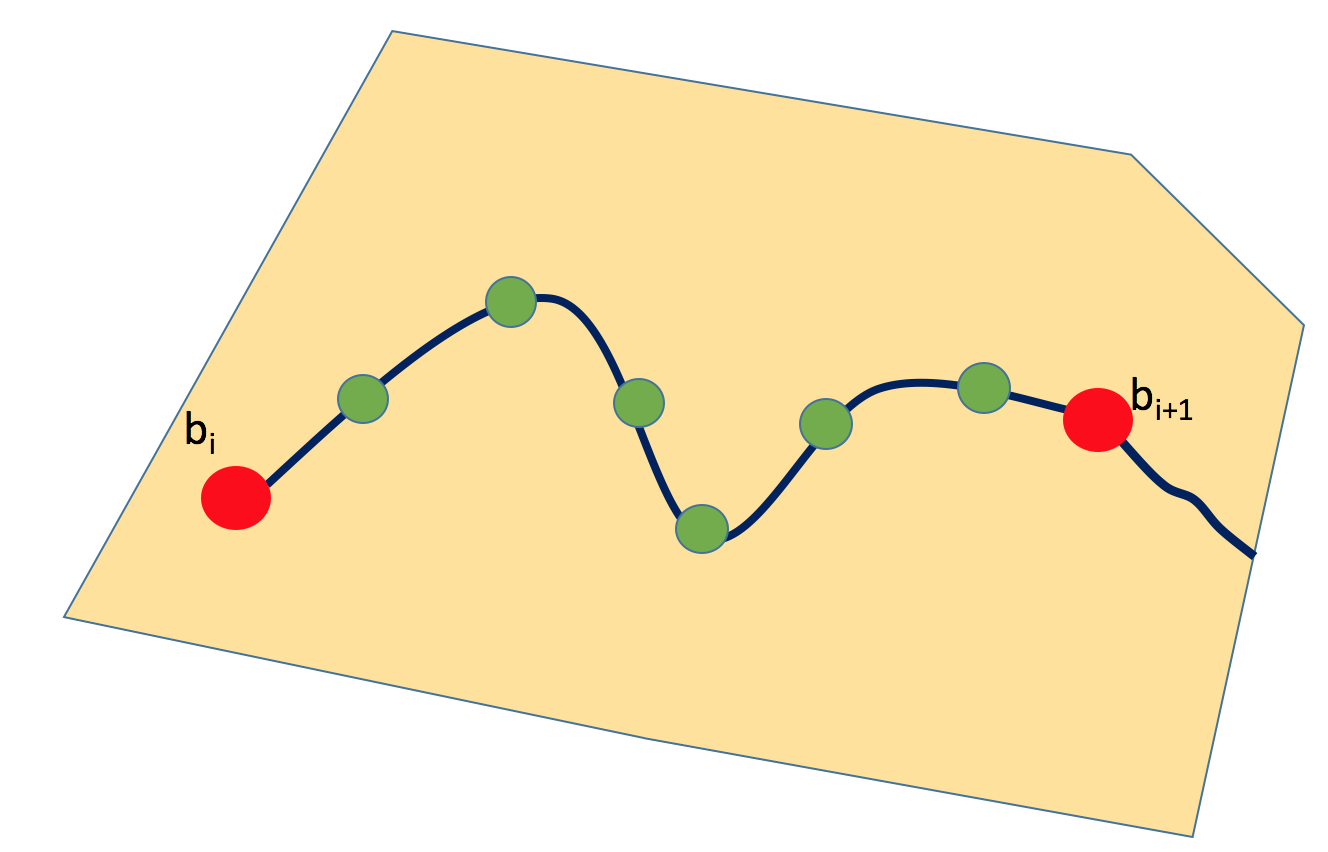
\includegraphics[width=0.5\textwidth]{img/puntiLinea}
	\caption{Esempio di campionamento di una linea ferroviaria } 
	\label{puntiLinea}
\end{figure}

\item nel caso in cui una tratta abbia una traiettoria complessa, il NMCE rileva tale situazione e provvede a dividere la linea in due o più linee semplici. In Fig.\ref{fig:divisioneLinea} un esempio esplicativo.

\begin{figure}[bth]
\myfloatalign
\subfloat[ Esempio di una linea ferroviaria complessa]
{\label{lineaComplessa}
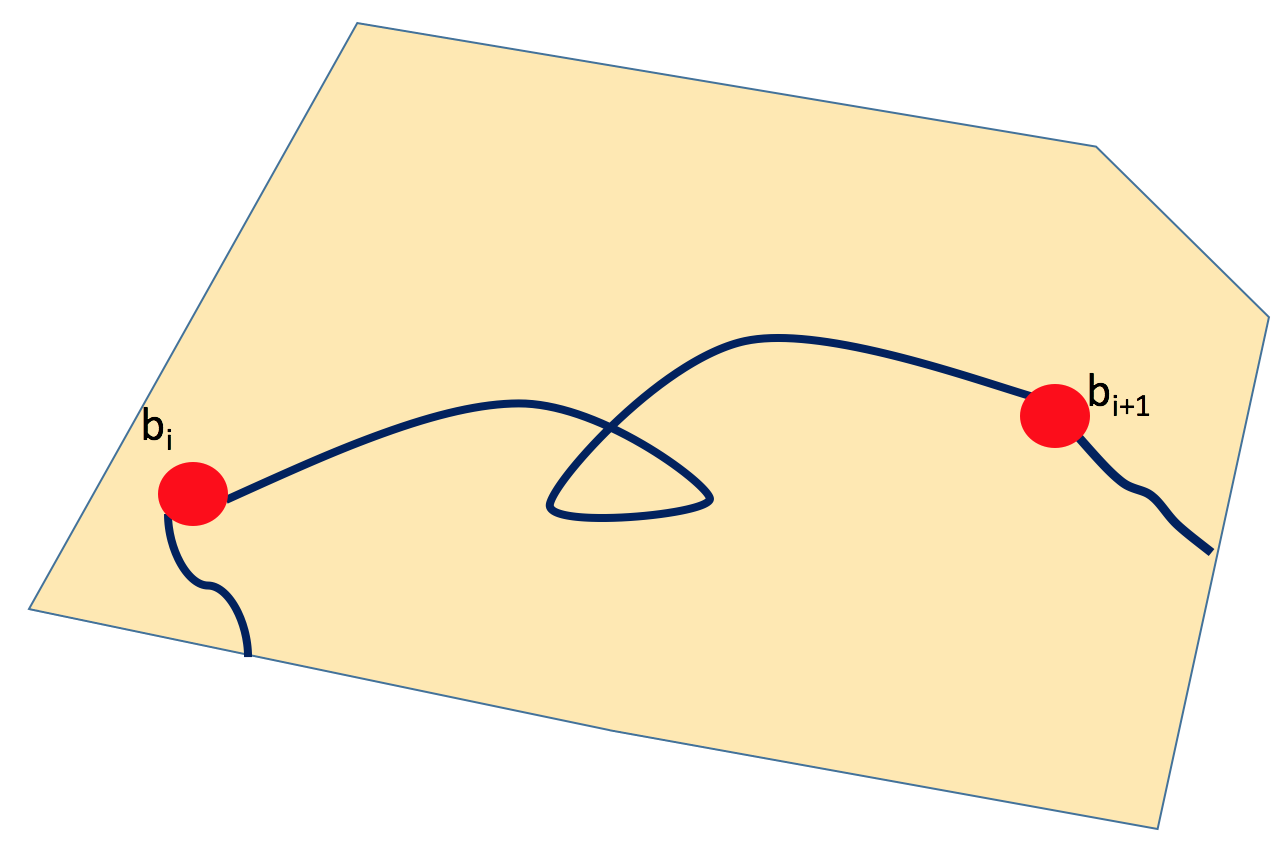
\includegraphics[width=.45\linewidth]{img/lineaComplessa}} \quad
\subfloat[ Esempio di linee semplici ottenute dividendo la linea in Fig. \ref{lineaComplessa}]
{\label{lineeSemplici}
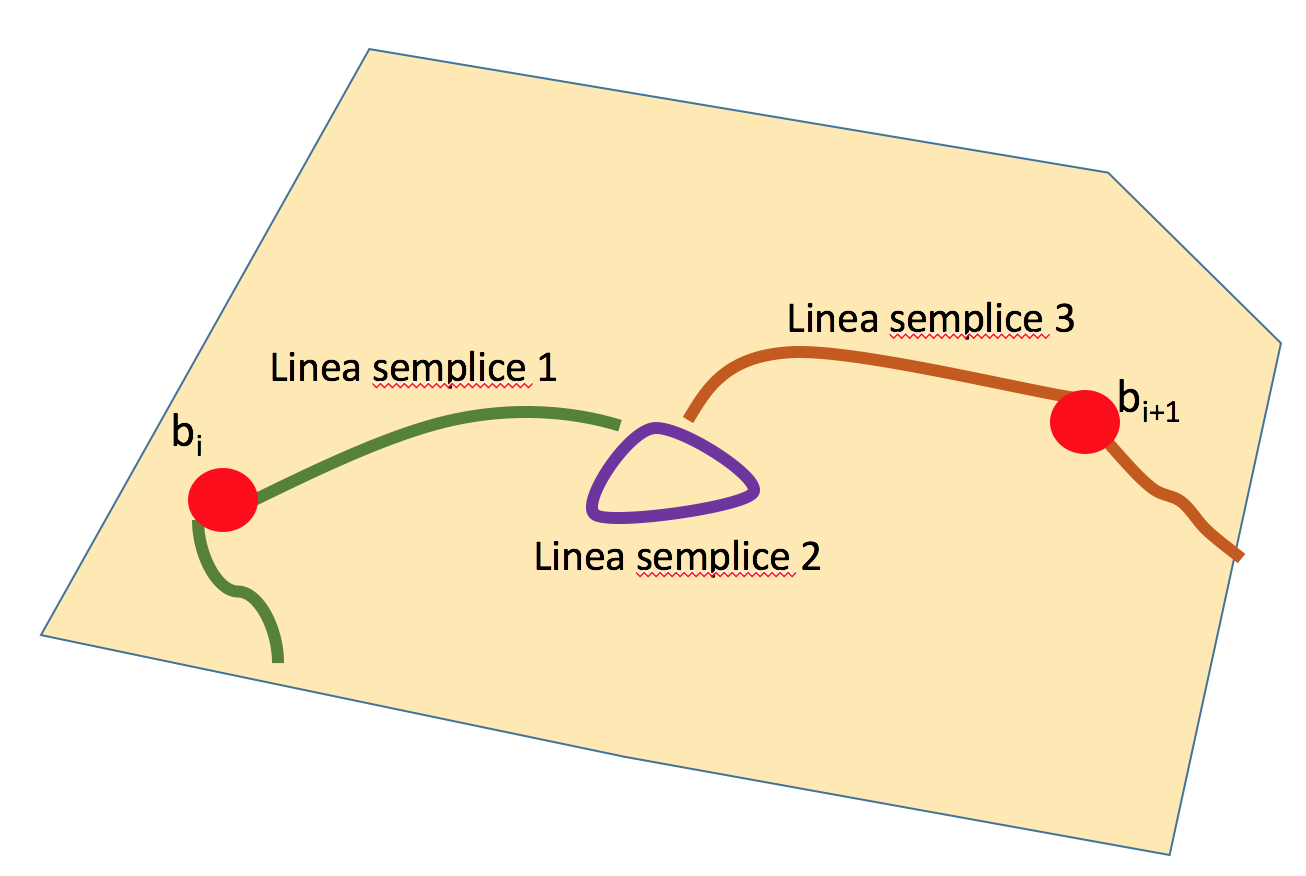
\includegraphics[width=.45\linewidth]{img/lineaSemplice}} 
\caption[dove]{Esempio di una linea ferroviaria complessa e della divisione in più linee semplici}
\label{fig:divisioneLinea}
\end{figure}
Come si evince dalla Fig.\ref{lineeSemplici}, la linea ferroviaria complessa in Fig.\ref{lineaComplessa} viene spezzata in tre linee semplici.

\item una volta campionata la tratta semplice, come in Fig.\ref{puntiLinea}, si utilizza il NMC per determinare il valore di \textit{exposure} di ogni punto che la compone. \newline
La linea ferroviaria viene quindi divisa in segmenti da 1 km ciascuno (fatta eccezione per l'ultimo segmento che potrebbe essere più piccolo) come in Fig.\ref{segmentiLinea}. Quindi il valore di \textit{exposure}  del segmento viene calcolato facendo la media aritmetica dell'\textit{exposure} dei punti campionati al suo interno. Di seguito in Fig.\ref{mediaExposure}  si propone un'esempio esplicativo, il colore del segmento tende sempre più al rosso all'aumentare del valore medio di \textit{exposure} dei punti contenuti nel segmento.

\begin{figure}[bth]
	\myfloatalign
	\subfloat[ Esempio di divisione ogni 1 km di una linea ferroviaria]
	{\label{segmentiLinea}
		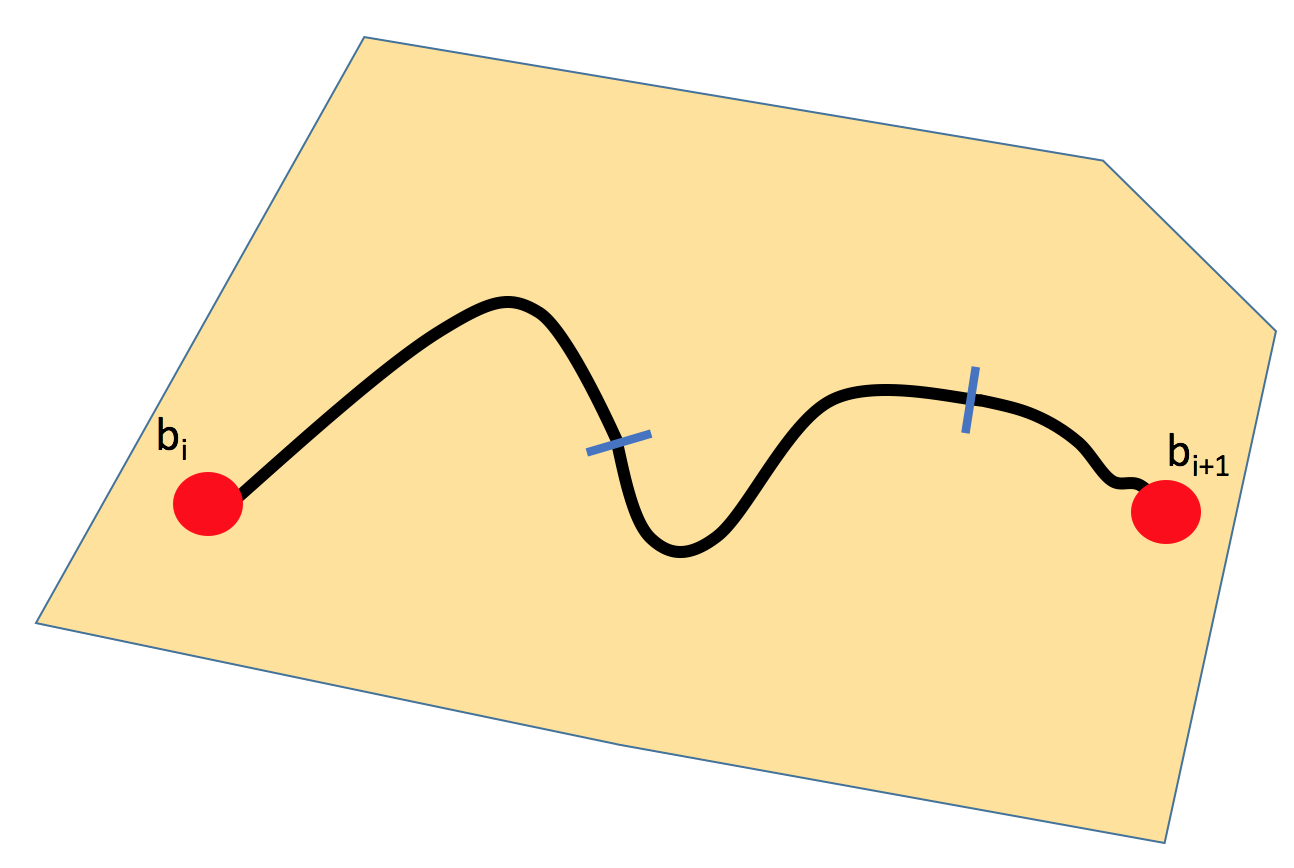
\includegraphics[width=.45\linewidth]{img/segmentiLinea}} \quad
	\subfloat[Esempio di assegnazione exposure per i segmenti di una linea ferroviaria ]
	{\label{mediaExposure}
		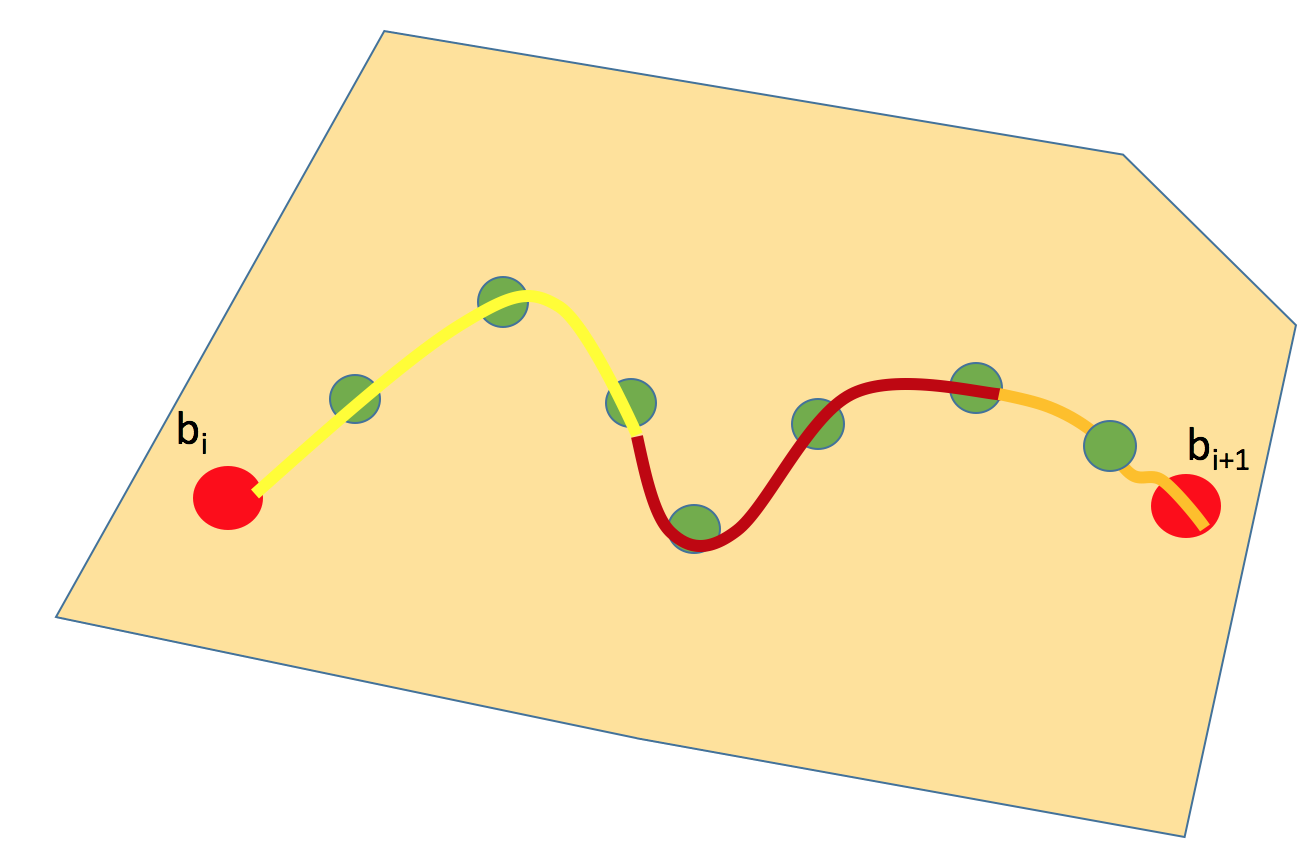
\includegraphics[width=.45\linewidth]{img/mediaExposure}} 
	\caption[dove]{Esempio di divisione ogni 1 km di una linea ferroviaria e assegnazione dell'exposure  ad ogni suo segmento }
	\label{fig:aggregazioneLinea}
\end{figure}


\end{enumerate}




\subsection{L'algoritmo}